% -*- Mode:TeX -*-

%% IMPORTANT: The official thesis specifications are available at:
%%            http://libraries.mit.edu/archives/thesis-specs/
%%
%%            Please verify your thesis' formatting and copyright
%%            assignment before submission.  If you notice any
%%            discrepancies between these templates and the 
%%            MIT Libraries' specs, please let us know
%%            by e-mailing thesis@mit.edu

%% The documentclass options along with the pagestyle can be used to generate
%% a technical report, a draft copy, or a regular thesis.  You may need to
%% re-specify the pagestyle after you \include  cover.tex.  For more
%% information, see the first few lines of mitthesis.cls. 

%\documentclass[12pt,vi,twoside]{mitthesis}
%%
%%  If you want your thesis copyright to you instead of MIT, use the
%%  ``vi'' option, as above.
%%
%\documentclass[12pt,twoside,leftblank]{mitthesis}
%%
%% If you want blank pages before new chapters to be labelled ``This
%% Page Intentionally Left Blank'', use the ``leftblank'' option, as
%% above. 
% Add all your packages here


\documentclass[12pt,twoside]{mitthesis}
\usepackage{enumerate}
\usepackage{graphicx}  
\def\spanishoptions{mexico}
\usepackage[spanish]{babel}
\usepackage[T1]{fontenc}
\usepackage[utf8]{inputenc}
\usepackage{amsmath} 
\usepackage{listings}
\usepackage{color}

\usepackage{caption}
\DeclareCaptionFormat{myformat}{#1#2#3}
\captionsetup{format=myformat}
\captionsetup[lstlisting]{position=bottom,format=myformat}
\renewcommand{\lstlistingname}{Algoritmo}

%\usepackage[T1,T2A]{fontenc}
%\usepackage[latin1]{inputenc}
%\usepackage[spanish]{babel}

%\selectlanguage{spanish}
\usepackage{lgrind}


\usepackage{fancyhdr}
\pagestyle{fancy}
\fancyhead{}
\fancyfoot{}
\fancyhead[RO,RE]{\fontsize{10}{12} \selectfont \thepage}
\fancyhead[LO]{\fontsize{10}{12} \selectfont \leftmark}
\fancyhead[LE]{\fontsize{10}{12} \selectfont \leftmark}

\addto\captionsspanish{%
  \renewcommand{\appendixname}%
    {Anexos}%
}
 
%% This bit allows you to either specify only the files which you wish to
%% process, or `all' to process all files which you \include.
%% Krishna Sethuraman (1990).

% \typein [\files]{Enter file names to process, (chap1,chap2 ...), or
%  `all' to process all files:}
\def\all{all}
% \ifx\files\all \typeout{Including all files.} \else \typeout{Including only \files.} \includeonly{\files} \fi

\begin{document}

% -*-latex-*-
% 
% For questions, comments, concerns or complaints:
% thesis@mit.edu
% 
%
% $Log: cover.tex,v $
% Revision 1.8  2008/05/13 15:02:15  jdreed
% Degree month is June, not May.  Added note about prevdegrees.
% Arthur Smith's title updated
%
% Revision 1.7  2001/02/08 18:53:16  boojum
% changed some \newpages to \cleardoublepages
%
% Revision 1.6  1999/10/21 14:49:31  boojum
% changed comment referring to documentstyle
%
% Revision 1.5  1999/10/21 14:39:04  boojum
% *** empty log message ***
%
% Revision 1.4  1997/04/18  17:54:10  othomas
% added page numbers on abstract and cover, and made 1 abstract
% page the default rather than 2.  (anne hunter tells me this
% is the new institute standard.)
%
% Revision 1.4  1997/04/18  17:54:10  othomas
% added page numbers on abstract and cover, and made 1 abstract
% page the default rather than 2.  (anne hunter tells me this
% is the new institute standard.)
%
% Revision 1.3  93/05/17  17:06:29  starflt
% Added acknowledgements section (suggested by tompalka)
% 
% Revision 1.2  92/04/22  13:13:13  epeisach
% Fixes for 1991 course 6 requirements
% Phrase "and to grant others the right to do so" has been added to 
% permission clause
% Second copy of abstract is not counted as separate pages so numbering works
% out
% 
% Revision 1.1  92/04/22  13:08:20  epeisach

% NOTE:
% These templates make an effort to conform to the MIT Thesis specifications,
% however the specifications can change.  We recommend that you verify the
% layout of your title page with your thesis advisor and/or the MIT 
% Libraries before printing your final copy.


\begin{titlepage}
  \begin{center}
    
\includegraphics[width=0.75\textwidth]{./logos.png}~\\[1cm]
    \textsc{\LARGE Optimización de textos publicitarios utilizando técnicas de computación evolutiva interactiva}~\\[0.5cm]
\textsc{por}~\\[0.5cm]
\textsc{\Large Elizabeth Quetzali Madera Hernández}~\\[2.0cm]

\textsc{\Large División de Estudios de Posgrado e Investigación}~\\[0.5cm]
\textsc{Tesis para obtener el grado de}~\\[0.5cm]
\textsc{\Large Maestra en Ciencias Computacionales}~\\[0.5cm]
\textsc{en el}~\\[0.5cm]
\textsc{\Large INSTITUTO TECNÓLOGICO DE TIJUANA}~\\[1cm]
\textsc{Julio 2014}~\\[0.2cm]
\textsc{Tijuana, Baja California, México}~\\[1cm]

\begin{minipage}{1.5\textwidth}
  \begin{flushleft} \large
    \emph{Director:}\\
    Dr. Jose Mario \textsc{García Valdez}
  \end{flushleft}
\end{minipage}

\begin{minipage}{1.5\textwidth}
\begin{flushleft} \large
\emph{Co-Directora:} \\
M.Cs. Alejandra \textsc{Mancilla Soto}
\end{flushleft}
\end{minipage}

\vfill

  \end{center}

\end{titlepage}

% Make the titlepage based on the above information.  If you need
% something special and can't use the standard form, you can specify
% the exact text of the titlepage yourself.  Put it in a titlepage
% environment and leave blank lines where you want vertical space.
% The spaces will be adjusted to fill the entire page.  The dotted
% lines for the signatures are made with the \signature command.
%\maketitle

% The abstractpage environment sets up everything on the page except
% the text itself.  The title and other header material are put at the
% top of the page, and the supervisors are listed at the bottom.  A
% new page is begun both before and after.  Of course, an abstract may
% be more than one page itself.  If you need more control over the
% format of the page, you can use the abstract environment, which puts
% the word "Abstract" at the beginning and single spaces its text.

%% You can either \input (*not* \include) your abstract file, or you can put
%% the text of the abstract directly between the \begin{abstractpage} and
%% \end{abstractpage} commands.

% First copy: start a new page, and save the page number.

% Uncomment the next line if you do NOT want a page number on your
% abstract and acknowledgments pages.
% \pagestyle{empty}
\setcounter{savepage}{\thepage}
\begin{abstractpage}
% $Log: abstract.tex,v $
% Revision 1.1  93/05/14  14:56:25  starflt
% Initial revision
% 
% Revision 1.1  90/05/04  10:41:01  lwvanels
% Initial revision
% 
%
%% The text of your abstract and nothing else (other than comments) goes here.
%% It will be single-spaced and the rest of the text that is supposed to go on
%% the abstract page will be generated by the abstractpage environment.  This
%% file should be \input (not \include 'd) from cover.tex.

La computación Evolutiva Interactiva (CEI) se utiliza en este trabajo con el fin de llevar a cabo la optimización de varios bloques de texto publicitarios. Los anuncios de texto siguen un formato similar al utilizado en una técnica llamada “Article Spinning”. Este formato permite que el algoritmo CEI evolucione el texto para un determinado grupo de personas, usando palabras y frases como partes variables que cambian de acuerdo a la evaluación subjetiva de la gente que interactúa con el algoritmo. Después de varias generaciones, el algoritmo de CEI da como resultado una versión del texto publicitario que, en teoría, debería exhibir un incremento en rendimiento, de acuerdo a la función de evaluación subjetiva con la cual fue evolucionado. Para poder demostrar la eficiencia de los textos, éstos son comparados contra una versión determinada por un experto en algún campo relacionado a la mercadotecnia. Para esta comparación, tres pruebas fueron realizadas: pruebas de memoria, reconocimiento, y persuasión. Los resultados obtenidos muestran que la CEI puede ser usada efectivamente para incrementar el impacto de un texto publicitario, pero más experimentos necesitan ser realizados.

\section*{Abstract}
Interactive Evolutionary Computation (IEC) is used in this work in order to perform the optimization of several advertisement blocks of text. The advertisement texts follow a format similar to the one used in a technique called Article Spinning. This format allows an IEC algorithm to evolve the text for a certain group of people, using words and phrases as variable parts which change according to the subjective evaluation of the people interacting with the algorithm. After several generations, the IEC algorithm provides a version of the advertisement text that, in theory, should exhibit an increased performance, according to the subjective evaluation function it was evolved with. In order to demonstrate the efficiency of the texts, these are compared against a version determined by an expert in a field related to marketing. For this comparison, three tests are performed: recall, recognition, and persuasion tests. The results obtained show that IEC could effectively be used to increase the impact of an advertisement text, but more experiments need to be conducted.

\end{abstractpage}

% Additional copy: start a new page, and reset the page number.  This way,
% the second copy of the abstract is not counted as separate pages.
% Uncomment the next 6 lines if you need two copies of the abstract
% page.
% \setcounter{page}{\thesavepage}
% \begin{abstractpage}
% % $Log: abstract.tex,v $
% Revision 1.1  93/05/14  14:56:25  starflt
% Initial revision
% 
% Revision 1.1  90/05/04  10:41:01  lwvanels
% Initial revision
% 
%
%% The text of your abstract and nothing else (other than comments) goes here.
%% It will be single-spaced and the rest of the text that is supposed to go on
%% the abstract page will be generated by the abstractpage environment.  This
%% file should be \input (not \include 'd) from cover.tex.

La computación Evolutiva Interactiva (CEI) se utiliza en este trabajo con el fin de llevar a cabo la optimización de varios bloques de texto publicitarios. Los anuncios de texto siguen un formato similar al utilizado en una técnica llamada “Article Spinning”. Este formato permite que el algoritmo CEI evolucione el texto para un determinado grupo de personas, usando palabras y frases como partes variables que cambian de acuerdo a la evaluación subjetiva de la gente que interactúa con el algoritmo. Después de varias generaciones, el algoritmo de CEI da como resultado una versión del texto publicitario que, en teoría, debería exhibir un incremento en rendimiento, de acuerdo a la función de evaluación subjetiva con la cual fue evolucionado. Para poder demostrar la eficiencia de los textos, éstos son comparados contra una versión determinada por un experto en algún campo relacionado a la mercadotecnia. Para esta comparación, tres pruebas fueron realizadas: pruebas de memoria, reconocimiento, y persuasión. Los resultados obtenidos muestran que la CEI puede ser usada efectivamente para incrementar el impacto de un texto publicitario, pero más experimentos necesitan ser realizados.

\section*{Abstract}
Interactive Evolutionary Computation (IEC) is used in this work in order to perform the optimization of several advertisement blocks of text. The advertisement texts follow a format similar to the one used in a technique called Article Spinning. This format allows an IEC algorithm to evolve the text for a certain group of people, using words and phrases as variable parts which change according to the subjective evaluation of the people interacting with the algorithm. After several generations, the IEC algorithm provides a version of the advertisement text that, in theory, should exhibit an increased performance, according to the subjective evaluation function it was evolved with. In order to demonstrate the efficiency of the texts, these are compared against a version determined by an expert in a field related to marketing. For this comparison, three tests are performed: recall, recognition, and persuasion tests. The results obtained show that IEC could effectively be used to increase the impact of an advertisement text, but more experiments need to be conducted.

% \end{abstractpage}

\cleardoublepage

\section*{Agradecimientos}

Quiero agradecer principalmente a mis cuatro mejores amigos:

Mi papá por todos sus sabios consejos que nunca me dejan desviar mi camino, por apoyarme en cualquier decisión que he tomado y por ser siempre mi héroe.

Mi mamá por demostrarme que una mujer puede acercarse mucho a la perfección si se lo propone y por enseñarme a ser autosuficiente.

Mi abuela por estar siempre disponible cuando la necesito y por todas esas platicas tan interesantes que me ha dado.

Mi novio Amaury por estar siempre a mi lado, por hacerme la mujer mas feliz del mundo y por ser mi profesor en muchas ocasiones.

Por haberme educado, haber creado una buena atmósfera donde pudiese crecer y por haber alimentado mi mente con sabiduría y amor, cualquier logro mío es también un logro de ustedes. Los amo con toda mi mente y mi corazón.

También quiero agradecer a todos mis profesores porque mi personalidad y mi forma de pensar están construidas con los pedacitos de conocimiento que me han brindado.

Muchas gracias Dr. Mario Garcia por su paciencia, conocimiento y orientación en cada paso que di durante mi investigacion, supo guiarme en todo momento.

Gracias M.Cs. Alejandra Mancilla por las sugerencias y aportaciones que me brindo cuando acudí a usted, fue de gran ayuda tenerla cerca porque aportaba ideas desde un punto de vista distinto al mío y al del Dr. Mario. Gracias a los dos porque fueron para mi un gran equipo.

Dra. Patricia Melin quiero agradecerle por inspirarme, conocer a una mujer que a llegado tan alto me da fuerzas para seguir estudiando. Usted es un gran ejemplo para mi.

Dr. Oscar Castillo gracias por su apoyo, su amabilidad y por sus consejos en cada seminario que fueron de gran ayuda y estimulo.

Gracias Dr. Jose Soria por sus correcciones y comentarios porque gracias a ellos pude entender con mayor profundidad la complejidad de algunos problemas que después pude resolver con mayor facilidad.

Me siento afortuna por haber tenido a tan buenos mentores. Es un orgullo decir que mi educación de posgrado fue impartida por ustedes.

Gracias desde el fondo de mi corazón a cada uno de ustedes. siempre ocuparan un lugar especial dentro de mi.


%%%%%%%%%%%%%%%%%%%%%%%%%%%%%%%%%%%%%%%%%%%%%%%%%%%%%%%%%%%%%%%%%%%%%%
% -*-latex-*-

% Some departments (e.g. 5) require an additional signature page.  See
% signature.tex for more information and uncomment the following line if
% applicable.
% % -*- Mode:TeX -*-
%
% Some departments (e.g. Chemistry) require an additional cover page
% with signatures of the thesis committee.  Please check with your
% thesis advisor or other appropriate person to determine if such a 
% page is required for your thesis.  
%
% If you choose not to use the "titlepage" environment, a \newpage
% commands, and several \vspace{\fill} commands may be necessary to
% achieve the required spacing.  The \signature command is defined in
% the "mitthesis" class
%
% The following sample appears courtesy of Ben Kaduk <kaduk@mit.edu> and
% was used in his June 2012 doctoral thesis in Chemistry. 

\begin{titlepage}
\begin{large}
This doctoral thesis has been examined by a Committee of the Department
of Chemistry as follows:

\signature{Professor Jianshu Cao}{Chairman, Thesis Committee \\
   Professor of Chemistry}

\signature{Professor Troy Van Voorhis}{Thesis Supervisor \\
   Associate Professor of Chemistry}

\signature{Professor Robert W. Field}{Member, Thesis Committee \\
   Haslam and Dewey Professor of Chemistry}
\end{large}
\end{titlepage}




  % -*- Mode:TeX -*-
%% This file simply contains the commands that actually generate the table of
%% contents and lists of figures and tables.  You can omit any or all of
%% these files by simply taking out the appropriate command.  For more
%% information on these files, see appendix C.3.3 of the LaTeX manual. 
\tableofcontents
\listoffigures
\listoftables


%% This is an example first chapter.  You should put chapter/appendix that you
%% write into a separate file, and add a line \include{yourfilename} to
%% main.tex, where `yourfilename.tex' is the name of the chapter/appendix file.
%% You can process specific files by typing their names in at the 
%% \files=
%% prompt when you run the file main.tex through LaTeX.

\chapter{Introducción}

El contenido textual es una parte fundamental para la publicidad en internet. Una buena elección de palabras es indispensable para la creación de un texto publicitario, de esto depende el sentido que se da al texto y afecta positiva o negativamente en el interés de los consumidores. Este trabajo presenta un método para la optimización de textos publicitarios mediante técnicas de computación evolutiva interactiva. 

El texto publicitario se divide en bloques de texto que al combinarlos se obtiene una gran cantidad de versiones de ese anuncio.

Los textos publicitarios pueden ser de longitud arbitraria, pero para los experimentos llevados a cabo se utilizan textos cortos. Para evolucionar un texto publicitario, primero se tiene que seguir un un formato propuesto por nosotros, descrito en la Sección 5.1. Este formato permite la representación de cada versión del texto en un cromosoma que puede ser utilizado por un algoritmo genético (ver Sección 3.3.1) para su evolución. 

Las distintas versiones del anuncio fueron presentadas a usuarios para que ellos eligieran la versión que más les atraía, las versiones fueron evolucionando en una plataforma llamada EvoSpace para obtener mediante la evolución una combinación que fuese más atractiva para la mayoría de los usuarios. 

\clearpage
\section{Descripción de la investigación}

Cuando se trata de comercio electrónico el texto toma un papel muy importante porque a través de el llevas la información del articulo en venta al consumidor. \cite{choi2002antecedents} El texto también puede ayudar a convencer al lector de comprar el producto que se anuncia. Cuando la persona encargada de el anuncio publicitario es un experto en el área, el producto obtiene mejores respuestas de los consumidores. La mezcla de las palabras o frases (bloques de texto) que los expertos deciden utilizar al escribir el texto es importante, porque esta mezcla puede ser la decisiva que provoque que el consumidor adquiera ese producto. Si un no experto desea escribir un anuncio publicitario seria muy difícil para él elegir la combinación correcta de los bloques de texto que serán de agrado para la mayoría de los consumidores, lo más factible seria escribir un texto que encierre el mensaje que quiere transmitir y dárselo a un experto para que este lo optimice segun su experiencia y sus conocimientos. 


Los algoritmos evolutivos son comúnmente usados para resolver problemas de optimización \cite{jong2006evolutionary} y es por eso que recurrimos a este método cuando nos interesamos en optimizar anuncios publicitarios. Creemos que si un grupo de personas puede evaluar distintas combinaciones del mismo anuncio, a través de varias generaciones se puede encontrar el anuncio optimo que sea del agrado de la mayoría de los consumidores.


\clearpage
\section{Objetivo General de la Investigación}

Se propone en este trabajo adaptar la plataforma EvoSpace-Interactivo para que optimice textos publicitarios, reescribiendo ciertos bloques de texto, con el fin de conseguir un texto que persuada más a comprar el producto, sea recordado y reconocido con mayor facilidad para la mayoría de  los usuarios.

Proponemos conseguir esta optimización a través de técnicas de computación evolutiva interactiva.

\clearpage
\section{Específicos de la Investigación}

Los objetivos específicos a desarrollar en este trabajo de investigación son los siguientes:

\begin{enumerate}
\item Adaptar la plataforma EvoSpace-Interactivo para optimizar textos publicitarios mediante técnicas de computación evolutiva interactiva.
\item Adaptar EvoSpace-Interactivo para la optimización de los textos publicitarios.
\item Comprobar que se puede optimizar el texto a través de técnicas de computación evolutiva interactiva para una población
\item Validar los resultados de los textos generados con nuestro método.
\item Analizar los resultados de los experimentos realizados.
\end{enumerate}

\clearpage
\section{Estructura del Documento de Tesis}

A continuación se explica brevemente el contenido de los siguientes capítulos que contiene esta tesis:

\begin{description}

\item[Capítulo 2] Se describe detalladamente el problema, las soluciones que existen actualmente y la solución propuesta.

\item[Capítulo 3] Se presenta algunos conceptos básicos para entender esta investigación y también partes esenciales que componen este proyecto como la plataforma utilizada que es una herramienta crucial para la implementación del algoritmo genético utilizado en esta investigación.

\item[Capítulo 4] Se incluyen los antecedentes de métodos utilizados para optimización de los distintos tipos de publicidad en internet,  ya que estos métodos son el fundamento para el desarrollo de este método propuesto.

\item[Capítulo 5] Se propone una arquitectura general para la optimización de textos, se describen y justifican los principales componentes y sus interacciones.

\item[Capítulo 6] Se detalla la implementación y adaptación de la plataforma EvoSpace-Interactivo, especificando las modificaciones realizadas. Se inicia el capitulo con una descripción breve del funcionamiento de de EvoSpace-Interactivo y la razón por la que es ideal para nuestra investigación.

\item[Capítulo 7] Se muestran los distintos experimentos realizado y sus  resultados.

\item[Capítulo 8] Se discuten los resultados y conclusiones sobre el trabajo expuesto, además se presentan propuestas para trabajos futuros.

\end{description}


%% This is an example first chapter.  You should put chapter/appendix that you
%% write into a separate file, and add a line \include{yourfilename} to
%% main.tex, where `yourfilename.tex' is the name of the chapter/appendix file.
%% You can process specific files by typing their names in at the 
%% \files=
%% prompt when you run the file main.tex through LaTeX.

\chapter{Descripción del problema}

El contenido textual es una parte fundamental para la publicidad en internet. Una buena elección de palabras es indispensable para la creación de un texto publicitario, de esto depende el sentido que se da al texto y afecta positiva o negativamente en el interés de los consumidores. El 97\% de los usuarios al encontrarse con sitios web nuevo escanean el texto que aparece para reconocer palabras y frases individuales con el fin de encontrar algo de interés.\cite{nielsen1997users} Como resultado, las páginas Web tienen que emplear texto susceptible de ser analizada utilizando conjuntos de palabras claves significativas que atraigan a los usuario. 

Contratar a un experto para crear contenido que pueda agradarle a la mayoría de los usuarios que entren a un sitio web puede ser una solución muy costosa, aun asi existe una creciente demanda de los escritores de contenido web especializados en Internet. Esto se debe a la calidad del contenido a menudo se traduce en mayores ingresos para los negocios en línea.\cite{kulkarni2014choose}

\section{Soluciones Existentes Actualmente}

Un escritor de contenido web es una persona que se especializa en la creación de contenido relevante para los sitios web. Cada sitio web tiene un publico objetivo especifico y requiere un un tipo de contenido. El contenido debe tener palabras clave que atraigan y retengan a los usuarios del sitio web. El contenido debe enfocarse en un tema especifico. El contenido generado debe ser considerado fácil de leer, informativo y agradable de leer. Normalmente se contrata a los escritores de contenido web para el desarrollo de contenido de sitios enfocados en la venta de artículos. En la tabla \ref{precios} se pueden observar los precios por palabra de las 10 empresas más populares dedicadas a la creación de contenido.

\begin{table}
\caption{Precios de compañías especializadas en creación de contenido web}
\label{precios}
\begin{center}
\begin{tabular}{|r|c|l|}
Compañia & Precio & Clasificación \\\hline \hline

Media Shower	 & \$49 dlls por publicación & ****\\
WriterAccess & \$50 dlls de depósito; de \$0.02 a \$1 por palabra & ****\\
CopyPress	 & \$5 dlls por 100 palabras & ****\\
Zerys	 & Los precios varian segun el proyecto & ***\\
Articlez & Los precios varian segun el proyecto & ***\\
SEO Article Writing Pros & Los precios varian segun el proyecto & ***\\
iWriter	 & Los precios varian segun el proyecto & ***\\
Constant Content	 & de \$20 a \$250 dlls dependiendo de la calidad & ***\\
Textbroker & de \$1.20 a \$6.70 cada 100 palabras & **\\
oDesk	 & Los precios varian segun el proyecto & *\\

\end{tabular}
\end{center}
\end{table}


\subsection{Solución Propuesta}

Este trabajo se presenta un método para la optimización de textos publicitarios mediante técnicas de computación evolutiva interactiva que pretende ser una solución más factible y alcanzable para la mayoría de interesados en el comercio electrónico.

El texto publicitario se divide en bloques de texto que al combinarlos se obtiene una gran cantidad de versiones de ese anuncio. Cada versión es representada por un vector que tiene la función de un cromosoma. Las distintas versiones del anuncio fuerón presentadas a usuarios para que ellos eligieran la versión que más les atraía, las versiones fueron evolucionando en una plataforma llamada EvoSpace para obtener mediante la evolución una combinación que fuese más atractiva para la mayoría de los usuarios. 

\section{Justificacion}

La razón para el desarrollo de la metodología propuesta en este trabajo es el potencial de reducir los costos monetarios en campañas de publicidad, el texto juega un papel muy importante en el comercio electrónico, ya que este es una de las formas más comunes de dar información acerca de un producto comercial a los consumidores \cite{mcquarrie1999visual}. Al desarrollar este método que optimiza textos publicitarios pretendemos principalmente alcanzar estas 3 metas:

\begin{enumerate}
\item Incrementar las ganancias del comercio electrónico personalizando las descripciones del  los productos para una población. 
\item Crear un nuevo método de optimización de anuncios.
\item Disminuir costos en campañas publicitarias
\end{enumerate}
%% This is an example first chapter.  You should put chapter/appendix that you
%% write into a separate file, and add a line \include{yourfilename} to
%% main.tex, where `yourfilename.tex' is the name of the chapter/appendix file.
%% You can process specific files by typing their names in at the 
%% \files=
%% prompt when you run the file main.tex through LaTeX.

\chapter{Conceptos Básicos}

\section{Publicidad en internet}

La publicidad en internet se hace a base del contenido de la pagina web. Para el desarrollo de este tipo de publicidad que tiene como fin dar a conocer por medio de este formato un producto a los usuarios en línea se incluyen elementos como texto, enlaces, imágenes, animaciones, etc. Existen compañías como Google que han creado sistemas para la publicad en internet en este caso AdSense y AdWords \cite{kowaliw2012promoting}, este sistema coloca la publicidad que se desea mostrar en los sitios relacionados con el tema del producto que se desea promocionar y se especifica el precio a pagar por cada clic del usuario a la publicidad. El sitio web que tiene anuncios al rededor de su contenido obtendrá ganancias según la cantidad de clics y el precio que se allá fijado para cada uno de los anuncios, El anunciante obtendrá mayor trafico en su sitio donde dispone del producto que anuncia, y así se logra la publicidad.

\section{Article spinning}

Article spinning es un método para crear múltiples versiones de un articulo sin crear versiones consideradas plagio ya que cada versión es única. El contenido duplicado no es aceptado por los motores de búsqueda como Google, Yahoo y Bing, así que este método se utiliza para generar muchos artículos basándose en uno solo, las palabras del articulo son sustituidas  por sinónimos automáticamente y se crea otra versión del articulo, esto ayuda a evitar las sanciones en las páginas de resultados de los motores de búsqueda ( SERP ) para el uso de contenido duplicado.\cite{takagi2001interactive}.

Existe gran similitud en el funcionamiento del "Article Spinning" con el de una máquina tragamonedas. Como se puede observar en la figura \ref{as}, podemos tener varias letras que pueden ser sustituidas en la primera ventana de la máquina tragamonedas. En este caso, esas letras son W, F y L, y representan bloques de texto. Al jalar la palanca, sólo una de de esas letras ganará la posición. La decisión de quién ganará la posición es aleatoria. Una vez que se jale la palanca (que sería el equivalente a accionar un botón para generar una combinación de palabras, y así crear un articulo nuevo) se genera una combinación de letras, que en este ejemplo fue la letra W, I y la letra N, las cuales juntas se puede leer como WIN (en español significa ganar).


\begin{figure}[htp]
  \centerline{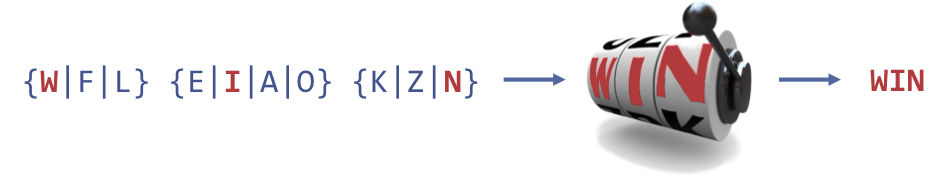
\includegraphics[width=4.5in]{as.png}} 
  \caption{funcionamiento del Article Spinning} 
\label{as}
\end{figure}


\section{Algoritmos Evolutivos}

Los algoritmos evolutivos son una rama de la inteligencia artificial, se utilizan principalmente en problemas con espacios de búsqueda muy extensos y no lineales. Estos algoritmos buscan soluciones basadas en la teoría de la evolución darwiniana. 
Con este método se mantiene un conjunto de individuos que representan posibles soluciones, estas soluciones se mezclan, y compiten entre si, de esa forma las soluciones mas aptas son capaces de sobrevivir a lo largo del tiempo y contribuir a las siguientes generaciones aportando sus genes, de esa forma estas generaciones venideras irán evolucionando hacia mejores soluciones cada vez. Existen distintos algoritmos evolutivos pero el que tiene mas importancia para esta investigación es el algoritmo genético da-do que es el que utilizamos para resolver nuestro problema.\cite{malcolm2008approach}

\subsection{Algoritmos Genéticos}

Los algoritmos genéticos (AG) (en la figura \ref{diagrama} podemos observar el diagrama de un AG) se inspiran en la evolución biológica, hacen evolucionar una población de individuos sometiéndola a mutaciones y recombinaciones genéticas, también a una selección de acuerdo a algún criterio, en función de este criterio se deciden cuales son los individuos más aptos, los cuales sobreviven y los menos aptos que son descartados. Es un método de búsqueda dirigida basada en probabilidad.\cite{back1996evolutionary}

Los algoritmos geneticos, consisten en una funcion matematica o una rutina que Simula el proceso evolutivo de las especies, teniendo como objetivo encontrar soluciones a problemas especificos de maximizacion o minimizacion. Asi, el algoritmo genetico recibe como entrada una generacion de posibles soluciones para el problema en cuestion, y arroja como salida los especimenes mas aptos (es decir, las mejores soluciones), para que se apareen y generen descendientes, los que deberian tener mejores caracteristicas que las generaciones anteriores.

Estos algoritmos mantienen elitismo ya que guarda siempre al mejor elemento de la población sin modificarlo. Al aumentar el numero de iteraciones, la probabilidad de encontrar el resultado optimo tiende a uno.

Los algoritmos geneticos trabajan con codigos que representan las posibles soluciones al problema. Por ello, es necesario establecer una codificacion para todo el rango de posibles soluciones antes de comenzar a trabajar con el algoritmo.La codificacion mas utilizada es la representacion de las soluciones por medio de cadenas binarias.\cite{parisi2004modelos}

\begin{figure}[htp]
  \centerline{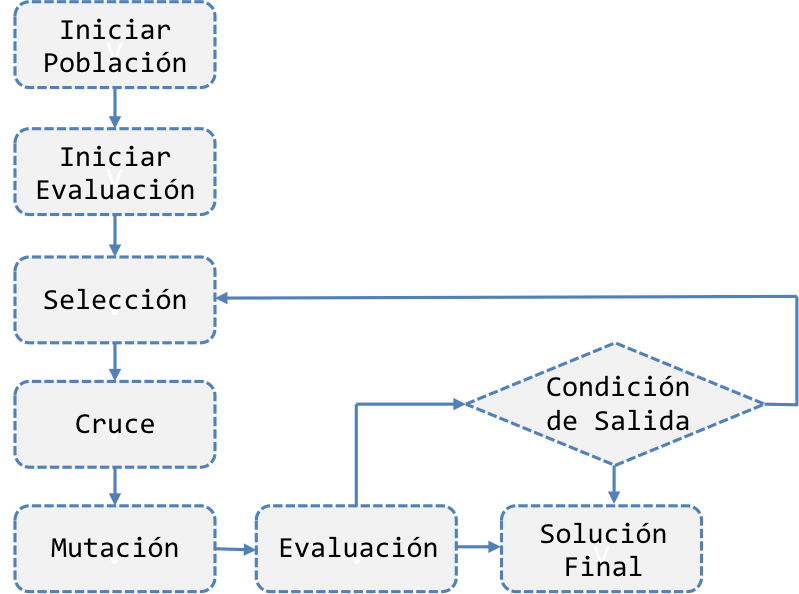
\includegraphics[width=4in]{diagrama.png}} 
  \caption{Diagrama de un Algoritmo Genético} 
\label{diagrama}
\end{figure}

\subsection{Computación Evolutiva Interactiva}

La computación evolutiva interactiva es una variación de la computación evolutiva en la cual la aptitud del individuo se determina mediante una evaluación subjetiva realizada por un usuario humano. En la computación tradicional, un humano requiere de un proceso computacional para resolver un problema, proporcionando la descripción del problema obtiene un resultado que después interpreta, pero en la computación evolutiva interactiva se invierten los papeles, existe un algoritmo que pide a un humano o a un grupo de humanos que resuelvan un problema, después recopila las soluciones para poder interpretarlas.\cite{dao2012novel}

Estos algoritmos se utilizan principalmente en problemas de optimización en el que el espacio de búsqueda es muy grande y complejo. Estos algoritmos de búsqueda de soluciones basadas en la teoría de la evolución darwiniana.
 
Este tipo de métodos de optimización generan un conjunto de individuos que representan posibles soluciones. Estas soluciones normalmente se generan al azar al comienzo del proceso de evolución. Después de cada generación, las mejores soluciones comparten parte de su información para crear otras posibles mejores soluciones. Todos los individuos compiten para ser la solución mas apta; las mejores soluciones se conservan, mientras que las peores son destruidos, de acuerdo con una función de aptitud que evalúa su rendimiento \cite{back1996evolutionary}. 

La computación evolutiva interactiva (CEI) utiliza una función de aptitud que se determina mediante la evaluación subjetiva de un ser humano, por ejemplo, una persona que está considerando un anuncio de texto para ser mejor que otro.

\section{EvoSpace}

Evospace es un espacio o hábitat en la nube donde se pueden almacenar y desarrollar algoritmos evolutivos. Evospace es muy versátil ya que la población es  independiente al modelo evolutivo que se pretenda utilizar. Los procesos clientes llamados EvoWorkes, interaccionan dinámica y asíncronamente, ellos también puede desplegarse en clientes remotos como en la plataforma que alberga al servidor.\cite{garcia2013evospace}
%% This is an example first chapter.  You should put chapter/appendix that you
%% write into a separate file, and add a line \include{yourfilename} to
%% main.tex, where `yourfilename.tex' is the name of the chapter/appendix file.
%% You can process specific files by typing their names in at the 
%% \files=
%% prompt when you run the file main.tex through LaTeX.

\chapter{Antecedentes}

En 2007, Kazienko y Adamski propusieron la extracción de patrones de usuario a través del uso de contenido web y técnicas de minería de uso web, y la creación de clusters en base a esta información \cite{kazienko2007adrosa}. Zheng, Chen, y Jiang, 2012, compararon el rendimiento de anuncios con sólo texto, sólo imágenes, y texto e imágenes, y concluyeron que no hay diferencia significativa entre sus rendimientos \cite{zheng2012ontology}. Keng y Liu, 2013, analizaron cómo es que los sitios web necesitan ser diseñados de acuerdo a la personalidad de los usuarios y sus intereses. \cite{keng2013can}. Wu, Zongda, et. al., 2013, se enfocaron en el posicionamiento óptimo de la publicidad, en lugar de la selección del anuncio para ser mostrado al usuario \cite{wu2013position}. Fan, Teng-Kai, y Chia-Hui Chang, 2011, propusieron un marco de trabajo de software para analizar el contenido de blogs, determinar el tema de su contenido, y recomendar anuncioos que fueran relevantes de acuerdo al contenido del blog \cite{fan2011blogger}. 

Dao, Tuan Hung, Seung Ryul Jeong, y Hyunchul Ahn, 2012, desarrollaron una herramiento que recomienda anuncios de acuerdo al contexto de un individuo. Usan la locación del usuario para proveer mejores anuncios. Su sistema de recomendación está basado en filtrado colaborativo \cite{dao2012novel}. Hsieh, Yu-Chen, y Kuo-Hsiang Chen, 2011, y Lewis, Whitler y Hoeg, 2013, estudiaron cómo el tipo de contenido (videos, texto, imágenes, o una mezcla de estos tipos) de un sitio web afectan la atención de un usuario hacia los anuncios de un sitio web \cite{hsieh2011different} \cite{lewis2013customer}. Finalmente, la prueba de persuación usada en este trabajo ha sido utilizada anteriormente en \cite{madera2014ad}.





%% This is an example first chapter.  You should put chapter/appendix that you
%% write into a separate file, and add a line \include{yourfilename} to
%% main.tex, where `yourfilename.tex' is the name of the chapter/appendix file.
%% You can process specific files by typing their names in at the 
%% \files=
%% prompt when you run the file main.tex through LaTeX.

\chapter{Arquitectura Propuesta}

\section{Formato del artículo}

El texto mostrado en la figura \ref{formato} esta formado por secciones encerradas entre llaves que pueden contener  bloques de texto. Los bloques de texto pueden ser de longitud arbitraria, puede abarcar desde una palabra hasta varios párrafos. Estos bloques de texto están divididos por barras, los bloques de texto que se encuentren fuera de los paréntesis (representados en color negro en la figura \ref{formato}) no tendrán ninguna alteración al evolucionar los textos.

\begin{figure}[htp]
  \centerline{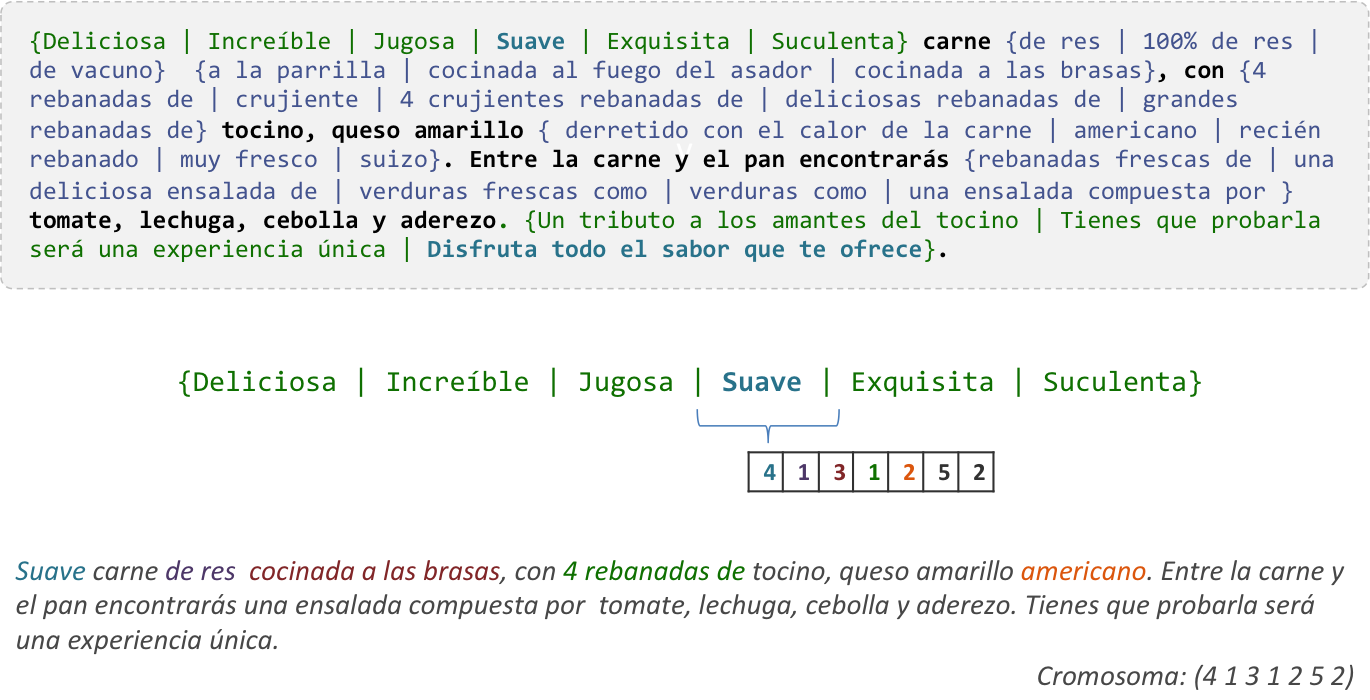
\includegraphics[width=6in]{formato.png}} 
  \caption{Formato del texto} 
\label{formato}
\end{figure}


El texto esta representado por un vector donde cada número indica la posición del bloque de texto al que se refiere, si la palabra que se quiere representar en la figura \ref{formato} es "Suave" entonces el vector indicará con el número 4 que la palabra se encuentra en la cuarta posición dentro de las opciones que el autor sugirió.


\clearpage
\section{Optimizacion del texto}

Se determinarán las mejores combinaciones utilizando un algoritmo genético, los pasos para evolucionar los textos generando nuevos individuos con mejores caracteristicas segun las elecciones de los usuarios son los siguientes.

\begin{enumerate}[\hspace*{0.5cm} P{a}so 1]
\item Se genera una población aleatoria de 100 individuos.
\item Se seleccionan 12 cromosomas, 6 del padre y 6 de la madre como se muestra en la figura \ref{padres}.

\begin{figure}[htp]
  \centerline{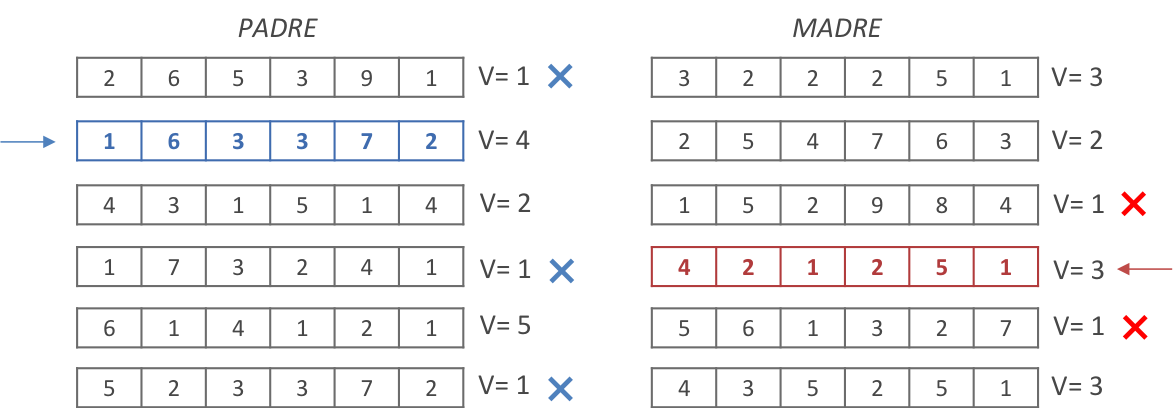
\includegraphics[width=6in]{padres.png}} 
  \caption{Seleccion de los cromosomas padres} 
\label{padres}
\end{figure}

\item Se calcula el fitness para seleccionar a los padres con mayor puntuación. La ecuación para calcular el ftiness es la siguiente:

\begin{equation}
Fitness = \frac{s+1 }{v+1 }   \textup{ donde }   \begin{matrix} \textup{ s = seleccion del texto} \\ \textup{ v = vistas del texto}\end{matrix}
\end{equation}

\item Se selecciona aleatoriamente  el tipo de cruce (los tipos de cruce se muestran en la figura \ref{cruce} ). La probabilidad de selección de alguno de los dos tipos de cruce es igual para ambos.

\begin{figure}[htp]
  \centerline{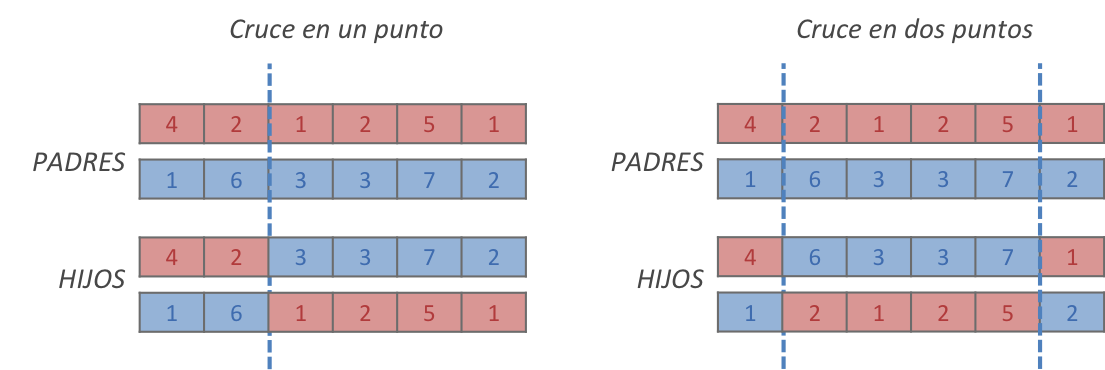
\includegraphics[width=6in]{cruce.png}} 
  \caption{Tipos de cruce utilizados} 
\label{cruce}
\end{figure}

\item Se crean dos nuevos cromosomas hijos. Hay una probabilidad del 10\% de que se efectúe una mutación para ambos cromosomas.
\item Se eliminan de la muestra los 2 cromosomas (un padre y una madre) con fitness más bajo y los hijos toman su lugar.
\end{enumerate}




%% This is an example first chapter.  You should put chapter/appendix that you
%% write into a separate file, and add a line \include{yourfilename} to
%% main.tex, where `yourfilename.tex' is the name of the chapter/appendix file.
%% You can process specific files by typing their names in at the 
%% \files=
%% prompt when you run the file main.tex through LaTeX.
\definecolor{mygray}{rgb}{0.95,0.95,0.96}
\definecolor{myblue}{rgb}{0.75,0.70,0.80}
\definecolor{mygreen}{rgb}{0.1,0.5,0.1}


\chapter{Adaptación de la Plataforma}


\section{Implementacion de EvoSpace-Interactivo}

Se modificó EvoSpace-Interactivo para poder evolucionar los textos publicitarios. El texto, en el formato explicado anteriormente, debe ser analizado para determinar cuántos segmentos de texto serán modificados, y cuáles son sus opciones. De esta forma se puede obtener un vector, que representaría la cromosoma de un individuo. EvoSpace crea 100 individuos aleatorios con los que se inicia la población. 

\clearpage
\subsection{Configuración del Sistema}

La plataforma evoSpace \cite{romero2014using} tuvo que ser modificado en varias áreas de su programación. Un nuevo módulo acepta un cromosoma como in-put, y produce una versión del anuncio de texto basados en el. Ahora la aplicación es capaz de mostrar texto en lugar de animaciones, como en la anterior aplicación llamada Shapes. 

La población se inicia con 100 individuos generados aleatoriamente. Para la evaluación de los individuos a los usuarios se le presentan dos textos  que una vez que el usuario elige el que mas llama su atención son regresados a EvoSpace, inmediatamente después se presentan otros dos textos listos para ser evaluados. Por cada par de muestras regresadas se comienza un proceso de apareamiento para poder agregar nuevos individuos a la población. El sistema esta operando en http://text.evospace.org.

A continuación en el Algoritmo 6.1 se muestra la sección de código encargada de delimitar el cromosoma a partir de el texto con el formato de Article Spinning. De esta manera el algoritmo no se ve afectado, no importa si el anuncio es muy pequeño o muy grande. 

La función options separa el texto según las opciones que contenga, pero lo transforma a un arreglo de Python. limit calcula cuál es el límite de cada uno de los genes del cromosoma. Si el imite es [5, 7, 9] al crear otro individuo aleatoriamente sabrá que puede elegir en la primera posición entre el número del 0 al 5, en la segunda del 0 al 7 y en la tercera posición del cromosoma del 0 al 9. limit\_ min te da un arreglo lleno de 0 de la longitud del texto.


\lstset{language=Python, breaklines=true, basicstyle=\footnotesize,  backgroundcolor=\color{mygray}}
\lstset{numbers=left, numberstyle=\tiny\color{red}, keywordstyle=\color{blue}, rulecolor=\color{myblue}, stringstyle=\color{mygreen},  stepnumber=1, numbersep=-6pt}

\begin{lstlisting}[frame=single]
  def options(txt):
      return [re.split("\s+?\|\s+?", position.strip("{}")) for position       in re.findall('{.+?}', txt)]

  def limit(txt):
      return [len(op) for op in options(txt)]

  def limit_min(txt):
      return [0 for tmp in limit(txt)]

  def init_pop(populationSize):
      text = "{Deliciosa | Increible | Jugosa | Suave | Exquisita |   Suculenta} carne {de res | 100% de res | de vacuno}  {a la parrilla | cocinada al fuego del asador | cocinada a las brasas}, con {4 rebanadas de | crujiente | 4 crujientes rebanadas de | deliciosas rebanadas de | grandes rebanadas de} tocino, queso amarillo { derretido con el calor de la carne | americano | recien rebanado | muy fresco | suizo}. Entre la carne y el pan encontraras {rebanadas frescas de | una deliciosa ensalada de | verduras frescas como | verduras como | una ensalada compuesta por } tomate, lechuga, cebolla y aderezo. {Un tributo a los amantes del tocino | Tienes que probarla sera una experiencia unica | Disfruta todo el sabor que te ofrece}."
    #populationSize = 5 #esta variable se recibe como parametro
    listSize = len(limit(text)) #esta variable se recibe como parametro
    chrome = [] #variable local
    limitmax = limit(text) #variable local
    limitmin = limit_min(text) #variable local
    
    server = Population()
    server.initialize()
    for individual in range(populationSize):
        for indice in range(listSize):
            aux = random.randint(limitmin[indice],limitmax[indice])
            chrome.insert(indice,aux)
        individual = {"id":None,"fitness":{"DefaultContext":0.0 },"chromosome":chrome,"views":0}
        server.put_individual(**individual)
        print chrome
        for x in chrome[:]: #inicializa la la lista
            chrome.remove(x)

\end{lstlisting}
\captionof{lstlisting}{Codigo que delimita el cromosona}

\clearpage
\section{Interfaz Gráfica}

En la figura \ref{interfaz} se muestra la adaptación de evoSpace para la evolución de los textos publicitarios. Dos versiones diferentes del texto se muestran al usuario en la parte inferior, una imagen del producto que se anuncia se muestra en el medio, y se muestra un botón para conseguir más versiones de texto en la esquina superior derecha.

Las características sociales de la plataforma no se muestra en esta adaptación, por lo que  los participantes no tienen la posibilidad de ser influenciados con las elecciones de los participantes anteriores. 

la cantidad de likes que se mostraba anteriormente fue eliminada al igual que las colecciones y la apariencia general de la interfaz gráfica se modifico para poder resaltar solo los textos; de esta forma el usuario solo se enfoca en la lectura sin que existan distracciones o influencias al momento de su elección.
 

\begin{figure}[htp]
  \centerline{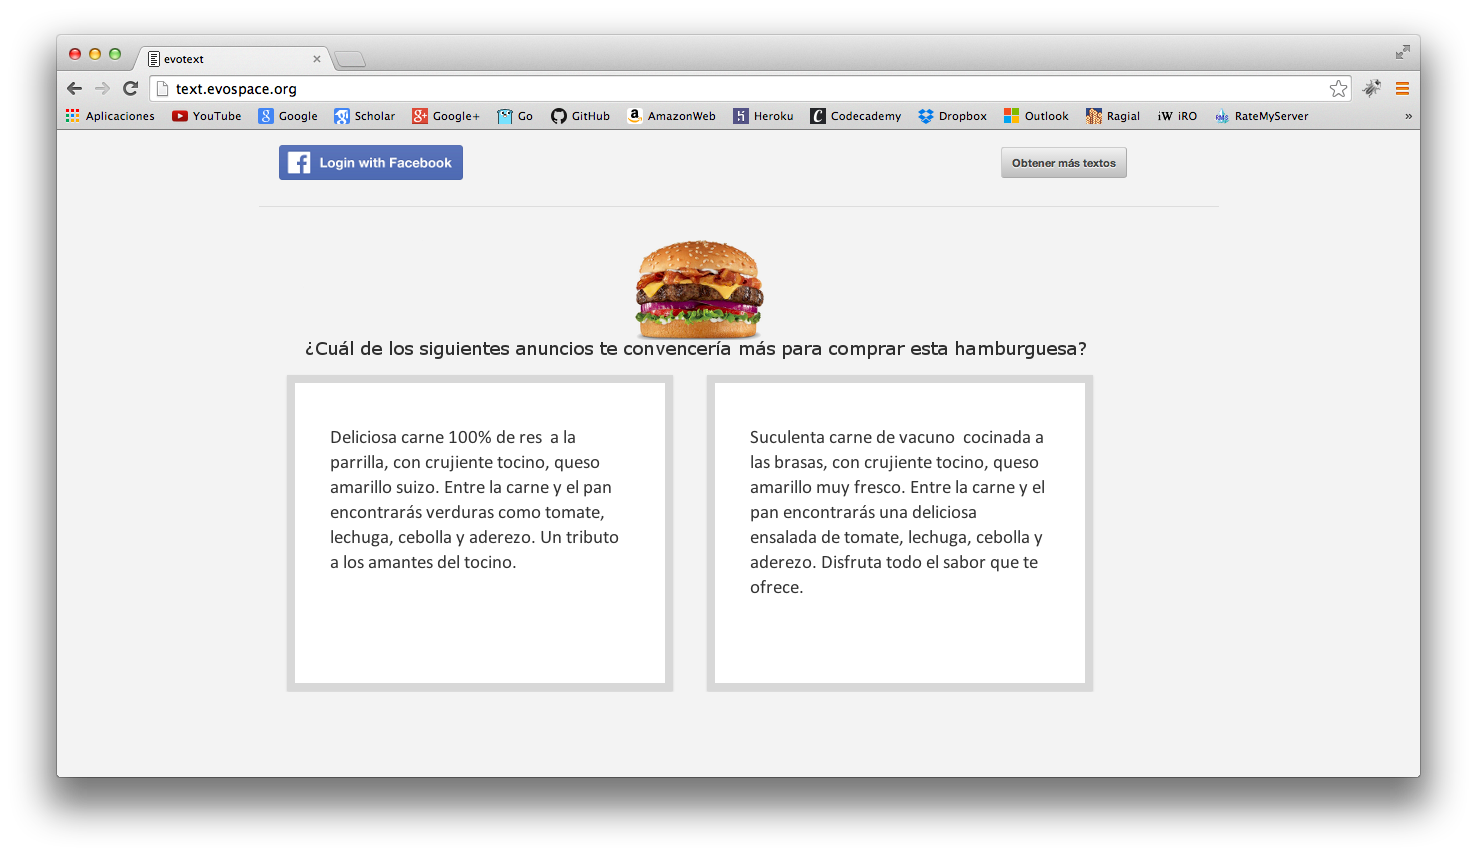
\includegraphics[width=7in]{interfaz.png}} 
  \caption{Interfaz Gráfica} 
\label{interfaz}
\end{figure}

\clearpage
\section{Eficiencia de un Anuncio Publicitario}

La efectividad de un anuncio esta relaciona con la atención que el usuario preste a dicho anuncio, para medir la atención se realizaron 2 pruebas basándonos en el trabajo de Yu-Chen Hsieh y Kuo-Hsiang Chen, 2010. Se realizaron pruebas de reconocimiento y de memoria. Añadimos una prueba para medir la persuasión del anuncio, se les preguntó a los participantes cuál anuncio, entre el generado y el hecho por un experto, creían que era el que más les convencía para comprar el producto que se anunciaba.
%% This is an example first chapter.  You should put chapter/appendix that you
%% write into a separate file, and add a line \include{yourfilename} to
%% main.tex, where `yourfilename.tex' is the name of the chapter/appendix file.
%% You can process specific files by typing their names in at the 
%% \files=
%% prompt when you run the file main.tex through LaTeX.

\chapter{Evaluación Experimental}

Inicialmente para comprobar este método se presentó a los usuarios una descripción de un anuncio de auto creado por Chevrolet y una descripción de una hamburguesa creada por Carl's Jr que eran comparados con dos anuncios creados por nuestro método, una descripción de un anuncio de un auto se comparaba con el anuncio de Chevrolet y una descripción de un anuncio de una hamburguesa se comparaba con el anuncio de Carl's Jr. Los resultados obtenidos fueron muy satisfactorios superando en preferencia del usuario el anuncio optimizado al anuncio creado por el experto. Con estos resultados pudimos darnos una idea del potencial de este método y continuar con las siguientes pruebas.

\clearpage
\section{El Método de Evaluación}

En nuestro método de evaluación la medición de la eficiencia de un anuncio de texto se realizó mediante la comparación de una versión que resultó de la evolución de los textos, contra una versión construida por un experto. Para los experimentos, una persona especializada en un área relacionada con el marketing es considerado un experto.
 
Para la primera parte del experimento, se le podio a un grupo de 30 personas, elegidas al azar, que eligiera la versión que ellos pensaban que podría persuadirlos con mayor facilidad. El texto con mayoría de votos se consideraba como el que más persuadía a una persona a comprar el producto anunciado. Aunque esta prueba podría presentar defectos, dado que la mejor estrategia para medir la efectividad de un anuncio de texto sería ponerlo en la práctica real, la prueba puede producir una idea aproximada de los resultados reales. 

Esta parte del experimento se repite con cinco versiones diferentes de diferentes expertos, contra el mismo texto evolucionado. 

La prueba de reconocimiento consiste en mostrar a un grupo de 30 personas el sitio web ficticio, donde se presenta un trailer de una película  durante 30 segundos. Por encima de este video, se muestra el texto del anuncio. Al terminar el video, el sitio web se oculto del participante, y se le pregunta a los participantes si vieron algún anuncio mientras miraban el video. Si los participantes vieron el anuncio, esto significa que reconocieron el anuncio. Al final, el número de personas que reconocieron el anuncio de texto se divide entre el total de participantes en esa prueba, lo que representa el porcentaje de reconocimiento para el anuncio dado. 

La prueba de memoria se realiza después de la prueba de reconocimiento. Al mismo grupo de personas que participaron en la prueba de reconocimiento, y que reconocieron con éxito el anuncio, se le pregunta si recuerdan de que trataba el anuncio. Al igual que en la prueba de reconocimiento, el número de personas que recordaron el tema del texto se divide entre el número total de participantes, lo que representa el porcentaje de memoria para el anuncio dado. 

El sitio web puede apreciarse en la Figura \ref{experimento}. El video se puede ver a la derecha, y el anuncio de texto en su parte superior, rodeado con un borde azul.

\begin{figure}[htp]
  \centerline{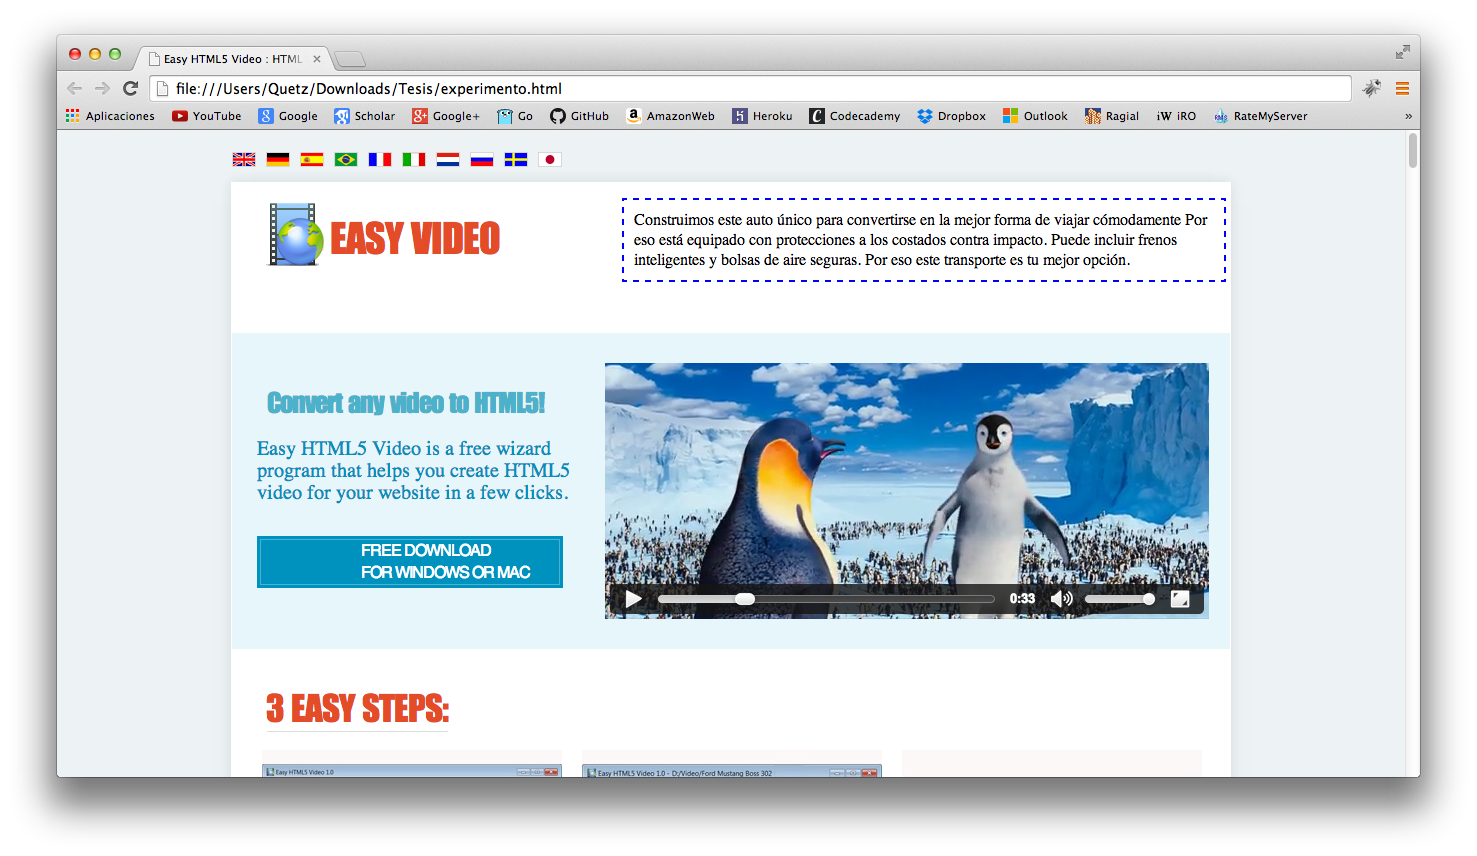
\includegraphics[width=7in]{experimento.png}} 
  \caption{Prueba de Reconocimiento y Memoria } 
\label{experimento}
\end{figure}

\clearpage
\section{Resultados}

La Tabla \ref{hamburgusa} presenta los resultados de los experimentos llevados a cabo utilizando el texto publicitario de la hamburguesa, mientras que la Tabla \ref{auto} se presentan los resultados del texto publicitario del automóvil.
Los porcentajes que se muestran en las tablas representan las calificaciones dadas por los participantes para cada versión de texto del anuncio. Por ejemplo,  el 60\%, significa que 60 personas de las 150 personas que participaron en el experimento, reconocía o recordaba el texto con éxito. En la prueba de la persuasión, los resultados son complementarios, lo que significa que, por ejemplo, el 56\% de los participantes prefirió la versión evolucionada del texto de la hamburguesa, mientras que el 44\% de los participantes prefirieron la versión del experto. 
Como se mencionó en la Sección 7.1, 30 personas participaron en cada parte del experimento. Se necesitaban 150 personas diferentes para cada prueba, ya que cada parte se realizó cinco veces (el texto evolucionado compitió contra cinco opciones diferentes expertos).

\begin{table}
\begin{center}
\begin{tabular}{|r|c|c|}
Tipo de Prueba & Promedio General (Evolucionado) & Promedio General (Experto) \\\hline \hline

Reconocimiento & 40\% & 46\% \\
Memoria & 27.3\% & 22\% \\
Persuasion & 56\% & 44\% \\

\end{tabular}
\end{center}
\caption{Resultados del experimento con el anuncio de la hamburguesa}
\label{hamburgusa}
\end{table}



\begin{table}
\begin{center}
\begin{tabular}{|r|c|c|}
Tipo de Prueba & Promedio General (Evolucionado) & Promedio General (Experto) \\\hline \hline

Reconocimiento & 65.3\% & 54.6\% \\
Memoria & 32.6\% & 24\% \\
Persuasion & 54\% & 46\% \\
\end{tabular}
\end{center}
\caption{Resultados del experimento con el anuncio del automóvil}
\label{auto}
\end{table}

\subsection{Tablas de resultados del anuncio del automóvil}

%1

\subsubsection{Nuestro Texto}

Diseñamos este carro único, para ser la mejor forma de viajar con tus amigos. Por eso está fabricado con barras laterales contra accidentes. Puede incluir frenos inteligentes y bolsas de aire seguras. Tiene transmisión automática de 4 velocidades.

\subsubsection{Texto del Experto}

Creamos este carro único, para que sea la mejor forma de viajar a donde quieras. Por eso está diseñado con barras laterales contra impacto. Puede incluir frenos antibloqueo y bolsas de aire seguras. Tiene transmisión automática de 4 velocidades.

\begin{table}
  \centering
  \tiny
\begin{tabular}{|r|c|c|c|c|c|c|}
   & \multicolumn{3}{c|}{Nuestro texto}     & \multicolumn{3}{c|}{Texto del experto}   \\\hline
   & Reconocimiento & Memoria & Persuación & Reconocimiento & Memoria & Persuación \\\hline \hline

1 &         1 &         1 &         0 &         1 &         1 &         1 \\
2 &         0 &         0 &         1 &         1 &         0 &         0 \\
3 &         0 &         0 &         1 &         1 &         1 &         0 \\
4 &         0 &         0 &         1 &         0 &         0 &         0 \\
5 &         0 &         0 &         1 &         0 &         0 &         0 \\
6 &         0 &         0 &         1 &         0 &         0 &         0 \\
7 &         1 &         1 &         1 &         1 &         0 &         0 \\
8 &         1 &         0 &         1 &         0 &         0 &         0 \\
9 &         1 &         1 &         0 &         1 &         0 &         1 \\
10 &         1 &         1 &         1 &         0 &         0 &         0 \\
11 &         1 &         1 &         0 &         1 &         1 &         1 \\
12 &         0 &         0 &         0 &         1 &         0 &         1 \\
13 &         1 &         0 &         0 &         0 &         0 &         1 \\
14 &         1 &         0 &         1 &         0 &         0 &         0 \\
15 &         1 &         0 &         0 &         0 &         0 &         1 \\
16 &         0 &         0 &         1 &         1 &         0 &         0 \\
17 &         1 &         0 &         0 &         0 &         0 &         1 \\
18 &         0 &         0 &         1 &         1 &         1 &         0 \\
19 &         0 &         0 &         0 &         0 &         0 &         1 \\
20 &         1 &         0 &         1 &         0 &         0 &         0 \\
21 &         1 &         0 &         1 &         0 &         0 &         0 \\
22 &         1 &         0 &         0 &         1 &         0 &         1 \\
23 &         1 &         1 &         0 &         1 &         0 &         1 \\
24 &         1 &         0 &         1 &         1 &         1 &         0 \\
25 &         1 &         0 &         1 &         1 &         1 &         0 \\
26 &         0 &         0 &         1 &         0 &         0 &         0 \\
27 &         1 &         0 &         1 &         1 &         1 &         0 \\
28 &         1 &         0 &         1 &         0 &         0 &         0 \\
29 &         1 &         1 &         0 &         0 &         0 &         1 \\
30 &         1 &         1 &         1 &         1 &         1 &         0 

\end{tabular}
\end{table}


%2

\subsubsection{Nuestro Texto}

Diseñamos este carro único, para ser la mejor forma de viajar con tus amigos. Por eso está fabricado con barras laterales contra accidentes. Puede incluir frenos inteligentes y bolsas de aire seguras. Tiene transmisión automática de 4 velocidades.

\subsubsection{Texto del Experto}

Creamos este carro único, para que sea la mejor forma de viajar a donde quieras. Por eso está diseñado con barras laterales contra impacto. Puede incluir frenos antibloqueo y bolsas de aire seguras. Tiene transmisión automática de 4 velocidades.

\begin{table}
  \centering
  \tiny
  \begin{tabular}{|r|c|c|c|c|c|c|}
   & \multicolumn{3}{c|}{Nuestro texto}     & \multicolumn{3}{c|}{Texto del experto}   \\\hline
   & Reconocimiento & Memoria & Persuación & Reconocimiento & Memoria & Persuación \\\hline \hline

1 &         0 &         0 &         1 &         0 &         0 &         0 \\
2 &         1 &         1 &         0 &         1 &         0 &         1 \\
3 &         1 &         0 &         1 &         1 &         0 &         0 \\
4 &         0 &         0 &         0 &         0 &         0 &         1 \\
5 &         1 &         1 &         0 &         0 &         0 &         1 \\
6 &         0 &         0 &         0 &         0 &         0 &         1 \\
7 &         0 &         0 &         0 &         1 &         1 &         1 \\
8 &         1 &         0 &         1 &         1 &         1 &         0 \\
9 &         1 &         1 &         0 &         1 &         0 &         1 \\
10 &         0 &         0 &         1 &         1 &         0 &         0 \\
11 &         0 &         0 &         1 &         0 &         0 &         0 \\
12 &         1 &         1 &         1 &         1 &         1 &         0 \\
13 &         1 &         1 &         1 &         0 &         0 &         0 \\
14 &         1 &         0 &         1 &         0 &         0 &         0 \\
15 &         1 &         1 &         1 &         1 &         0 &         0 \\
16 &         0 &         0 &         0 &         0 &         0 &         1 \\
17 &         1 &         1 &         1 &         1 &         1 &         0 \\
18 &         1 &         1 &         1 &         1 &         1 &         0 \\
19 &         0 &         0 &         1 &         1 &         0 &         0 \\
20 &         1 &         1 &         1 &         0 &         0 &         0 \\
21 &         1 &         0 &         0 &         1 &         0 &         1 \\
22 &         1 &         0 &         0 &         0 &         0 &         1 \\
23 &         0 &         0 &         0 &         1 &         0 &         1 \\
24 &         0 &         0 &         0 &         1 &         0 &         1 \\
25 &         1 &         1 &         1 &         0 &         0 &         0 \\
26 &         0 &         0 &         1 &         1 &         1 &         0 \\
27 &         1 &         1 &         0 &         1 &         0 &         1 \\
28 &         0 &         0 &         1 &         1 &         1 &         0 \\
29 &         1 &         1 &         1 &         1 &         1 &         0 \\
30 &         0 &         0 &         0 &         1 &         0 &         1 

\end{tabular}
\end{table}


%3

\subsubsection{Nuestro Texto}

Diseñamos este carro único, para ser la mejor forma de viajar con tus amigos. Por eso está fabricado con barras laterales contra accidentes. Puede incluir frenos inteligentes y bolsas de aire seguras. Tiene transmisión automática de 4 velocidades.

\subsubsection{Texto del Experto}

Creamos este carro único, para que sea la mejor forma de viajar a donde quieras. Por eso está diseñado con barras laterales contra impacto. Puede incluir frenos antibloqueo y bolsas de aire seguras. Tiene transmisión automática de 4 velocidades.

\begin{table}
\centering
\tiny
\begin{tabular}{|r|c|c|c|c|c|c|}
   & \multicolumn{3}{c|}{Nuestro texto}     & \multicolumn{3}{c|}{Texto del experto}   \\\hline
   & Reconocimiento & Memoria & Persuación & Reconocimiento & Memoria & Persuación \\\hline \hline

1 &         1 &         1 &         1 &         0 &         0 &         0 \\
2 &         1 &         0 &         1 &         1 &         0 &         0 \\
3 &         1 &         0 &         0 &         0 &         0 &         1 \\
4 &         0 &         0 &         0 &         1 &         1 &         1 \\
5 &         0 &         0 &         1 &         1 &         0 &         0 \\
6 &         0 &         0 &         0 &         1 &         1 &         1 \\
7 &         0 &         0 &         0 &         1 &         0 &         1 \\
8 &         1 &         0 &         0 &         0 &         0 &         1 \\
9 &         1 &         0 &         1 &         1 &         0 &         0 \\
10 &         1 &         0 &         1 &         0 &         0 &         0 \\
11 &         1 &         0 &         1 &         1 &         1 &         0 \\
12 &         1 &         0 &         1 &         1 &         0 &         0 \\
13 &         1 &         1 &         0 &         1 &         0 &         1 \\
14 &         1 &         1 &         1 &         1 &         0 &         0 \\
15 &         1 &         0 &         0 &         0 &         0 &         1 \\
16 &         1 &         1 &         1 &         1 &         0 &         0 \\
17 &         1 &         1 &         0 &         0 &         0 &         1 \\
18 &         1 &         0 &         1 &         1 &         1 &         0 \\
19 &         0 &         0 &         0 &         0 &         0 &         1 \\
20 &         0 &         0 &         1 &         0 &         0 &         0 \\
21 &         1 &         1 &         0 &         0 &         0 &         1 \\
22 &         0 &         0 &         1 &         0 &         0 &         0 \\
23 &         0 &         0 &         1 &         0 &         0 &         0 \\
24 &         1 &         1 &         1 &         1 &         1 &         0 \\
25 &         1 &         0 &         0 &         1 &         1 &         1 \\
26 &         1 &         0 &         1 &         0 &         0 &         0 \\
27 &         1 &         0 &         0 &         1 &         0 &         1 \\
28 &         1 &         1 &         1 &         1 &         0 &         0 \\
29 &         1 &         1 &         0 &         0 &         0 &         1 \\
30 &         1 &         0 &         0 &         1 &         0 &         1 

\end{tabular}
\end{table}


%4

\subsubsection{Nuestro Texto}

Diseñamos este carro único, para ser la mejor forma de viajar con tus amigos. Por eso está fabricado con barras laterales contra accidentes. Puede incluir frenos inteligentes y bolsas de aire seguras. Tiene transmisión automática de 4 velocidades.

\subsubsection{Texto del Experto}

Creamos este carro único, para que sea la mejor forma de viajar a donde quieras. Por eso está diseñado con barras laterales contra impacto. Puede incluir frenos antibloqueo y bolsas de aire seguras. Tiene transmisión automática de 4 velocidades.

\begin{table}
\centering
\tiny
\begin{tabular}{|r|c|c|c|c|c|c|}
   & \multicolumn{3}{c|}{Nuestro texto}     & \multicolumn{3}{c|}{Texto del experto}   \\\hline
   & Reconocimiento & Memoria & Persuación & Reconocimiento & Memoria & Persuación \\\hline \hline

1 &         1 &         0 &         1 &         1 &         0 &         0 \\
2 &         1 &         1 &         0 &         0 &         0 &         1 \\
3 &         1 &         0 &         1 &         1 &         0 &         0 \\
4 &         1 &         0 &         0 &         1 &         0 &         1 \\
5 &         1 &         0 &         1 &         1 &         1 &         0 \\
6 &         1 &         0 &         0 &         1 &         1 &         1 \\
7 &         1 &         0 &         0 &         0 &         0 &         1 \\
8 &         1 &         0 &         0 &         1 &         1 &         1 \\
9 &         1 &         1 &         0 &         0 &         0 &         1 \\
10 &         1 &         1 &         1 &         0 &         0 &         0 \\
11 &         0 &         0 &         0 &         0 &         0 &         1 \\
12 &         1 &         0 &         1 &         0 &         0 &         0 \\
13 &         1 &         1 &         1 &         0 &         0 &         0 \\
14 &         0 &         0 &         0 &         0 &         0 &         1 \\
15 &         1 &         0 &         0 &         1 &         0 &         1 \\
16 &         0 &         0 &         0 &         1 &         0 &         1 \\
17 &         0 &         0 &         0 &         0 &         0 &         1 \\
18 &         1 &         1 &         0 &         0 &         0 &         1 \\
19 &         1 &         1 &         0 &         1 &         1 &         1 \\
20 &         1 &         0 &         1 &         0 &         0 &         0 \\
21 &         1 &         0 &         1 &         1 &         0 &         0 \\
22 &         1 &         1 &         1 &         1 &         1 &         0 \\
23 &         1 &         0 &         1 &         0 &         0 &         0 \\
24 &         1 &         0 &         1 &         1 &         1 &         0 \\
25 &         0 &         0 &         0 &         0 &         0 &         1 \\
26 &         1 &         1 &         0 &         0 &         0 &         1 \\
27 &         1 &         1 &         1 &         1 &         0 &         0 \\
28 &         1 &         1 &         0 &         1 &         1 &         1 \\
29 &         0 &         0 &         0 &         1 &         0 &         1 \\
30 &         0 &         0 &         0 &         0 &         0 &         1 

\end{tabular}
\end{table}

%5

\subsubsection{Nuestro Texto}

Diseñamos este carro único, para ser la mejor forma de viajar con tus amigos. Por eso está fabricado con barras laterales contra accidentes. Puede incluir frenos inteligentes y bolsas de aire seguras. Tiene transmisión automática de 4 velocidades.

\subsubsection{Texto del Experto}

Creamos este carro único, para que sea la mejor forma de viajar a donde quieras. Por eso está diseñado con barras laterales contra impacto. Puede incluir frenos antibloqueo y bolsas de aire seguras. Tiene transmisión automática de 4 velocidades.

\begin{table}
\centering
\tiny
\begin{tabular}{|r|c|c|c|c|c|c|}
   & \multicolumn{3}{c|}{Nuestro texto}     & \multicolumn{3}{c|}{Texto del experto}   \\\hline
   & Reconocimiento & Memoria & Persuación & Reconocimiento & Memoria & Persuación \\\hline \hline

1 &         0 &         0 &         1 &         1 &         0 &         0 \\
2 &         0 &         0 &         0 &         0 &         0 &         1 \\
3 &         0 &         0 &         0 &         0 &         0 &         1 \\
4 &         1 &         1 &         0 &         0 &         0 &         1 \\
5 &         0 &         0 &         1 &         0 &         0 &         0 \\
6 &         1 &         1 &         1 &         0 &         0 &         0 \\
7 &         1 &         1 &         1 &         1 &         0 &         0 \\
8 &         1 &         0 &         0 &         0 &         0 &         1 \\
9 &         1 &         0 &         0 &         1 &         0 &         1 \\
10 &         0 &         0 &         1 &         1 &         1 &         0 \\
11 &         0 &         0 &         1 &         1 &         1 &         0 \\
12 &         1 &         0 &         1 &         0 &         0 &         0 \\
13 &         1 &         1 &         1 &         1 &         1 &         0 \\
14 &         0 &         0 &         0 &         1 &         1 &         1 \\
15 &         0 &         0 &         0 &         0 &         0 &         1 \\
16 &         1 &         0 &         0 &         1 &         0 &         1 \\
17 &         0 &         0 &         1 &         0 &         0 &         0 \\
18 &         0 &         0 &         1 &         1 &         1 &         0 \\
19 &         1 &         0 &         0 &         1 &         0 &         1 \\
20 &         0 &         0 &         1 &         0 &         0 &         0 \\
21 &         1 &         1 &         0 &         1 &         0 &         1 \\
22 &         1 &         1 &         1 &         1 &         0 &         0 \\
23 &         1 &         0 &         1 &         1 &         0 &         0 \\
24 &         1 &         1 &         1 &         0 &         0 &         0 \\
25 &         0 &         0 &         0 &         0 &         0 &         1 \\
26 &         1 &         1 &         1 &         0 &         0 &         0 \\
27 &         0 &         0 &         1 &         1 &         0 &         0 \\
28 &         1 &         1 &         0 &         1 &         1 &         1 \\
29 &         1 &         1 &         1 &         0 &         0 &         0 \\
30 &         0 &         0 &         0 &         1 &         1 &         1 

\end{tabular}
\end{table}



\subsection{Tablas de resultados del anuncio de la hamburguesa}

%H1

\subsubsection{Nuestro Texto}

Jugosa carne de vacuno  a la parrilla, con crujiente tocino, queso amarillo  derretido con el calor de la carne. Entre la carne y el pan encontrarás verduras frescas como tomate, lechuga, cebolla y aderezo. Tienes que probarla será una experiencia única.

\subsubsection{Texto del Experto}

Exquisita carne de vacuno  cocinada a las brasas, con deliciosas rebanadas de tocino, queso amarillo suizo. Entre la carne y el pan encontrarás una deliciosa ensalada de tomate, lechuga, cebolla y aderezo. Tienes que probarla será una experiencia única.

\begin{table}
\centering
\tiny
\begin{tabular}{|r|c|c|c|c|c|c|}
   & \multicolumn{3}{c|}{Nuestro texto}     & \multicolumn{3}{c|}{Texto del experto}   \\\hline
   & Reconocimiento & Memoria & Persuación & Reconocimiento & Memoria & Persuación \\\hline \hline

1 &         0 &         0 &         0 &         0 &         0 &         1 \\
2 &         0 &         0 &         0 &         0 &         0 &         1 \\
3 &         1 &         1 &         1 &         1 &         1 &         0 \\
4 &         0 &         0 &         1 &         0 &         0 &         0 \\
5 &         0 &         0 &         0 &         1 &         1 &         1 \\
6 &         0 &         0 &         1 &         1 &         1 &         0 \\
7 &         1 &         1 &         1 &         0 &         0 &         0 \\
8 &         0 &         0 &         1 &         1 &         1 &         0 \\
9 &         1 &         1 &         0 &         0 &         0 &         1 \\
10 &         0 &         0 &         0 &         0 &         0 &         1 \\
11 &         1 &         0 &         0 &         0 &         0 &         1 \\
12 &         1 &         1 &         1 &         1 &         0 &         0 \\
13 &         0 &         0 &         1 &         0 &         0 &         0 \\
14 &         1 &         1 &         1 &         1 &         1 &         0 \\
15 &         1 &         1 &         1 &         0 &         0 &         0 \\
16 &         0 &         0 &         1 &         0 &         0 &         0 \\
17 &         1 &         1 &         0 &         0 &         0 &         1 \\
18 &         0 &         0 &         0 &         0 &         0 &         1 \\
19 &         0 &         0 &         0 &         0 &         0 &         1 \\
20 &         0 &         0 &         1 &         0 &         0 &         0 \\
21 &         0 &         0 &         0 &         1 &         0 &         1 \\
22 &         1 &         1 &         0 &         0 &         0 &         1 \\
23 &         0 &         0 &         0 &         1 &         1 &         1 \\
24 &         0 &         0 &         1 &         1 &         0 &         0 \\
25 &         1 &         1 &         0 &         1 &         0 &         1 \\
26 &         0 &         0 &         1 &         0 &         0 &         0 \\
27 &         1 &         1 &         0 &         0 &         0 &         1 \\
28 &         0 &         0 &         1 &         0 &         0 &         0 \\
29 &         0 &         0 &         1 &         1 &         1 &         0 \\
30 &         0 &         0 &         0 &         1 &         1 &         1 

\end{tabular}
\end{table}

%H2

\subsubsection{Nuestro Texto}

Jugosa carne de vacuno  a la parrilla, con crujiente tocino, queso amarillo  derretido con el calor de la carne. Entre la carne y el pan encontrarás verduras frescas como tomate, lechuga, cebolla y aderezo. Tienes que probarla será una experiencia única.

\subsubsection{Texto del Experto}

Exquisita carne de vacuno  cocinada a las brasas, con deliciosas rebanadas de tocino, queso amarillo suizo. Entre la carne y el pan encontrarás una deliciosa ensalada de tomate, lechuga, cebolla y aderezo. Tienes que probarla será una experiencia única.

\begin{table}
\centering
\tiny
\begin{tabular}{|r|c|c|c|c|c|c|}
   & \multicolumn{3}{c|}{Nuestro texto}     & \multicolumn{3}{c|}{Texto del experto}   \\\hline
   & Reconocimiento & Memoria & Persuación & Reconocimiento & Memoria & Persuación \\\hline \hline

1 &         1 &         1 &         1 &         0 &         0 &         0 \\
2 &         0 &         0 &         1 &         0 &         0 &         0 \\
3 &         1 &         0 &         0 &         0 &         0 &         1 \\
4 &         1 &         1 &         1 &         1 &         1 &         0 \\
5 &         0 &         0 &         0 &         1 &         1 &         1 \\
6 &         1 &         1 &         1 &         1 &         1 &         0 \\
7 &         0 &         0 &         1 &         1 &         1 &         0 \\
8 &         0 &         0 &         1 &         0 &         0 &         0 \\
9 &         0 &         0 &         0 &         0 &         0 &         1 \\
10 &         0 &         0 &         1 &         0 &         0 &         0 \\
11 &         0 &         0 &         0 &         0 &         0 &         1 \\
12 &         1 &         1 &         1 &         0 &         0 &         0 \\
13 &         1 &         0 &         1 &         1 &         1 &         0 \\
14 &         1 &         0 &         0 &         1 &         1 &         1 \\
15 &         0 &         0 &         0 &         1 &         0 &         1 \\
16 &         1 &         1 &         1 &         1 &         1 &         0 \\
17 &         1 &         1 &         0 &         0 &         0 &         1 \\
18 &         0 &         0 &         1 &         0 &         0 &         0 \\
19 &         0 &         0 &         1 &         0 &         0 &         0 \\
20 &         0 &         0 &         1 &         0 &         0 &         0 \\
21 &         0 &         0 &         1 &         0 &         0 &         0 \\
22 &         0 &         0 &         1 &         1 &         1 &         0 \\
23 &         1 &         0 &         0 &         0 &         0 &         1 \\
24 &         0 &         0 &         1 &         0 &         0 &         0 \\
25 &         0 &         0 &         1 &         1 &         1 &         0 \\
26 &         0 &         0 &         0 &         1 &         1 &         1 \\
27 &         1 &         1 &         1 &         1 &         0 &         0 \\
28 &         0 &         0 &         0 &         0 &         0 &         1 \\
29 &         1 &         1 &         0 &         1 &         1 &         1 \\
30 &         1 &         0 &         1 &         0 &         0 &         0 

\end{tabular}
\end{table}


%H3

\subsubsection{Nuestro Texto}

Jugosa carne de vacuno  a la parrilla, con crujiente tocino, queso amarillo  derretido con el calor de la carne. Entre la carne y el pan encontrarás verduras frescas como tomate, lechuga, cebolla y aderezo. Tienes que probarla será una experiencia única.

\subsubsection{Texto del Experto}

Exquisita carne de vacuno  cocinada a las brasas, con deliciosas rebanadas de tocino, queso amarillo suizo. Entre la carne y el pan encontrarás una deliciosa ensalada de tomate, lechuga, cebolla y aderezo. Tienes que probarla será una experiencia única.

\begin{table}
\centering
\tiny
\begin{tabular}{|r|c|c|c|c|c|c|}
   & \multicolumn{3}{c|}{Nuestro texto}     & \multicolumn{3}{c|}{Texto del experto}   \\\hline
   & Reconocimiento & Memoria & Persuación & Reconocimiento & Memoria & Persuación \\\hline \hline

1 &         1 &         1 &         0 &         0 &         0 &         1 \\
2 &         0 &         0 &         1 &         1 &         0 &         0 \\
3 &         0 &         0 &         0 &         0 &         0 &         1 \\
4 &         0 &         0 &         1 &         0 &         0 &         0 \\
5 &         0 &         0 &         0 &         1 &         0 &         1 \\
6 &         1 &         1 &         0 &         0 &         0 &         1 \\
7 &         0 &         0 &         1 &         0 &         0 &         0 \\
8 &         1 &         1 &         1 &         1 &         1 &         0 \\
9 &         0 &         0 &         1 &         1 &         1 &         0 \\
10 &         0 &         0 &         1 &         0 &         0 &         0 \\
11 &         1 &         1 &         1 &         1 &         0 &         0 \\
12 &         0 &         0 &         0 &         0 &         0 &         1 \\
13 &         1 &         1 &         1 &         1 &         0 &         0 \\
14 &         1 &         1 &         0 &         0 &         0 &         1 \\
15 &         0 &         0 &         1 &         1 &         0 &         0 \\
16 &         0 &         0 &         0 &         1 &         0 &         1 \\
17 &         0 &         0 &         0 &         0 &         0 &         1 \\
18 &         1 &         1 &         0 &         1 &         0 &         1 \\
19 &         1 &         1 &         0 &         0 &         0 &         1 \\
20 &         0 &         0 &         1 &         0 &         0 &         0 \\
21 &         0 &         0 &         1 &         1 &         1 &         0 \\
22 &         0 &         0 &         1 &         0 &         0 &         0 \\
23 &         0 &         0 &         1 &         1 &         1 &         0 \\
24 &         0 &         0 &         0 &         0 &         0 &         1 \\
25 &         1 &         1 &         0 &         0 &         0 &         1 \\
26 &         0 &         0 &         0 &         1 &         0 &         1 \\
27 &         0 &         0 &         1 &         0 &         0 &         0 \\
28 &         1 &         0 &         0 &         0 &         0 &         1 \\
29 &         0 &         0 &         0 &         0 &         0 &         1 \\
30 &         0 &         0 &         0 &         1 &         1 &         1 

\end{tabular}
\end{table}


%H4

\subsubsection{Nuestro Texto}

Jugosa carne de vacuno  a la parrilla, con crujiente tocino, queso amarillo  derretido con el calor de la carne. Entre la carne y el pan encontrarás verduras frescas como tomate, lechuga, cebolla y aderezo. Tienes que probarla será una experiencia única.

\subsubsection{Texto del Experto}

Exquisita carne de vacuno  cocinada a las brasas, con deliciosas rebanadas de tocino, queso amarillo suizo. Entre la carne y el pan encontrarás una deliciosa ensalada de tomate, lechuga, cebolla y aderezo. Tienes que probarla será una experiencia única.

\begin{table}
\centering
\tiny
\begin{tabular}{|r|c|c|c|c|c|c|}
   & \multicolumn{3}{c|}{Nuestro texto}     & \multicolumn{3}{c|}{Texto del experto}   \\\hline
   & Reconocimiento & Memoria & Persuación & Reconocimiento & Memoria & Persuación \\\hline \hline

1 &         1 &         0 &         0 &         1 &         1 &         1 \\
2 &         0 &         0 &         1 &         1 &         0 &         0 \\
3 &         0 &         0 &         1 &         0 &         0 &         0 \\
4 &         1 &         1 &         0 &         1 &         0 &         1 \\
5 &         0 &         0 &         0 &         0 &         0 &         1 \\
6 &         0 &         0 &         1 &         0 &         0 &         0 \\
7 &         1 &         1 &         0 &         0 &         0 &         1 \\
8 &         1 &         0 &         0 &         1 &         0 &         1 \\
9 &         0 &         0 &         1 &         0 &         0 &         0 \\
10 &         1 &         1 &         0 &         1 &         0 &         1 \\
11 &         0 &         0 &         1 &         0 &         0 &         0 \\
12 &         1 &         1 &         0 &         1 &         0 &         1 \\
13 &         1 &         0 &         1 &         0 &         0 &         0 \\
14 &         0 &         0 &         1 &         0 &         0 &         0 \\
15 &         0 &         0 &         0 &         1 &         0 &         1 \\
16 &         1 &         0 &         0 &         1 &         0 &         1 \\
17 &         0 &         0 &         0 &         1 &         1 &         1 \\
18 &         1 &         1 &         1 &         1 &         0 &         0 \\
19 &         0 &         0 &         0 &         1 &         0 &         1 \\
20 &         1 &         0 &         1 &         1 &         0 &         0 \\
21 &         0 &         0 &         1 &         1 &         1 &         0 \\
22 &         1 &         1 &         1 &         0 &         0 &         0 \\
23 &         0 &         0 &         1 &         1 &         1 &         0 \\
24 &         1 &         1 &         1 &         0 &         0 &         0 \\
25 &         0 &         0 &         0 &         0 &         0 &         1 \\
26 &         0 &         0 &         0 &         0 &         0 &         1 \\
27 &         0 &         0 &         1 &         0 &         0 &         0 \\
28 &         0 &         0 &         1 &         1 &         0 &         0 \\
29 &         0 &         0 &         1 &         1 &         0 &         0 \\
30 &         0 &         0 &         1 &         0 &         0 &         0 

\end{tabular}
\end{table}


%H5

\subsubsection{Nuestro Texto}

Jugosa carne de vacuno  a la parrilla, con crujiente tocino, queso amarillo  derretido con el calor de la carne. Entre la carne y el pan encontrarás verduras frescas como tomate, lechuga, cebolla y aderezo. Tienes que probarla será una experiencia única.

\subsubsection{Texto del Experto}

Exquisita carne de vacuno  cocinada a las brasas, con deliciosas rebanadas de tocino, queso amarillo suizo. Entre la carne y el pan encontrarás una deliciosa ensalada de tomate, lechuga, cebolla y aderezo. Tienes que probarla será una experiencia única.

\begin{table}
\centering
\tiny
\begin{tabular}{|r|c|c|c|c|c|c|}
   & \multicolumn{3}{c|}{Nuestro texto}     & \multicolumn{3}{c|}{Texto del experto}   \\\hline
   & Reconocimiento & Memoria & Persuación & Reconocimiento & Memoria & Persuación \\\hline \hline

1 &         1 &         1 &         1 &         1 &         0 &         0 \\
2 &         0 &         0 &         1 &         0 &         0 &         0 \\
3 &         0 &         0 &         0 &         1 &         1 &         1 \\
4 &         1 &         0 &         1 &         1 &         0 &         0 \\
5 &         0 &         0 &         1 &         1 &         1 &         0 \\
6 &         1 &         0 &         1 &         0 &         0 &         0 \\
7 &         1 &         1 &         0 &         1 &         1 &         1 \\
8 &         0 &         0 &         0 &         0 &         0 &         1 \\
9 &         1 &         1 &         0 &         0 &         0 &         1 \\
10 &         0 &         0 &         1 &         1 &         0 &         0 \\
11 &         0 &         0 &         0 &         0 &         0 &         1 \\
12 &         1 &         1 &         0 &         1 &         0 &         1 \\
13 &         1 &         0 &         1 &         0 &         0 &         0 \\
14 &         1 &         1 &         1 &         1 &         0 &         0 \\
15 &         1 &         0 &         1 &         0 &         0 &         0 \\
16 &         1 &         0 &         0 &         0 &         0 &         1 \\
17 &         0 &         0 &         1 &         1 &         1 &         0 \\
18 &         0 &         0 &         1 &         1 &         0 &         0 \\
19 &         0 &         0 &         0 &         0 &         0 &         1 \\
20 &         0 &         0 &         1 &         1 &         0 &         0 \\
21 &         0 &         0 &         1 &         0 &         0 &         0 \\
22 &         1 &         0 &         0 &         0 &         0 &         1 \\
23 &         0 &         0 &         1 &         0 &         0 &         0 \\
24 &         1 &         1 &         0 &         1 &         0 &         1 \\
25 &         0 &         0 &         1 &         0 &         0 &         0 \\
26 &         0 &         0 &         1 &         1 &         0 &         0 \\
27 &         1 &         0 &         1 &         0 &         0 &         0 \\
28 &         0 &         0 &         1 &         1 &         0 &         0 \\
29 &         0 &         0 &         1 &         1 &         1 &         0 \\
30 &         1 &         1 &         0 &         0 &         0 &         1 

\end{tabular}
\end{table}
%% This is an example first chapter.  You should put chapter/appendix that you
%% write into a separate file, and add a line \include{yourfilename} to
%% main.tex, where `yourfilename.tex' is the name of the chapter/appendix file.
%% You can process specific files by typing their names in at the 
%% \files=
%% prompt when you run the file main.tex through LaTeX.

\chapter{Conclusiones y Trabajo Futuro}


\section{Conclusiones}

Evolucionar textos publicitarios partiendo de una descripción realizada por un inexperto en el área de mercadotecnia es una gran alternativa para crear textos publicitarios con una respuesta favorable por los posibles consumidores. Aun Deben realizarse más experimentos con el fin de obtener resultados más confiables. También, los resultados presentados demuestran que el método propuesto en este trabajo puede potencialmente ayudar en el desarrollo de una campaña de marketing.
Sin duda la optimización de los textos publicitarios es una herramienta importante que se debe considerar para futuras campañas de marketing.


\section{Trabajo Futuro}

Se esta trabajando en la implementación de un algoritmo de clustering k-means para agrupar a los usuarios según su perfil y evolucionar los anuncios para cada grupo de usuarios con el fin de generar anuncios optimizados tomando en cuenta las preferencias de los distintos tipos de consumidores.
\appendix
%% This defines the bibliography file (main.bib) and the bibliography style.
%% If you want to create a bibliography file by hand, change the contents of
%% this file to a `thebibliography' environment.  For more information 
%% see section 4.3 of the LaTeX manual.
\begin{singlespace}
\bibliography{main}
\bibliographystyle{plain}
\end{singlespace}

\chapter{ }

\begin{figure}[htp]
  \centerline{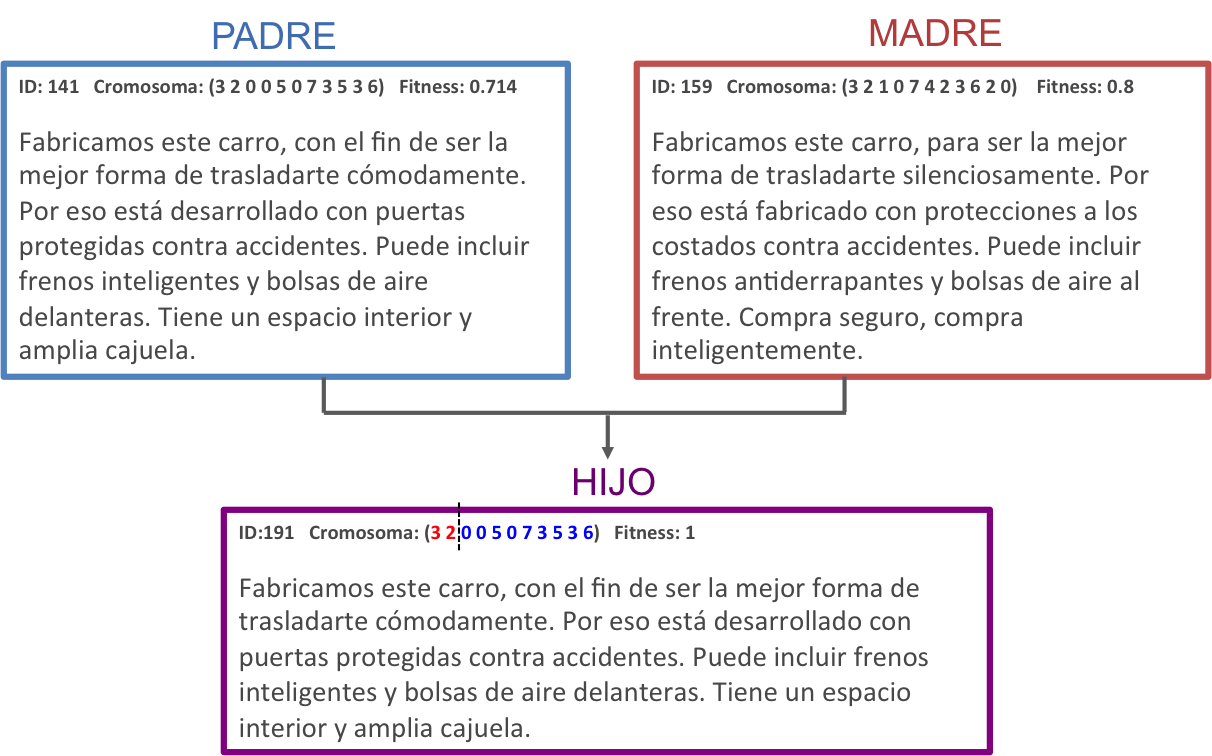
\includegraphics[width=7in]{h.png}} 
  \caption{Árbol Genealógico de un cromosoma (Parte del Hijo)} 
\label{h}
\end{figure}

\begin{figure}[htp]
  \centerline{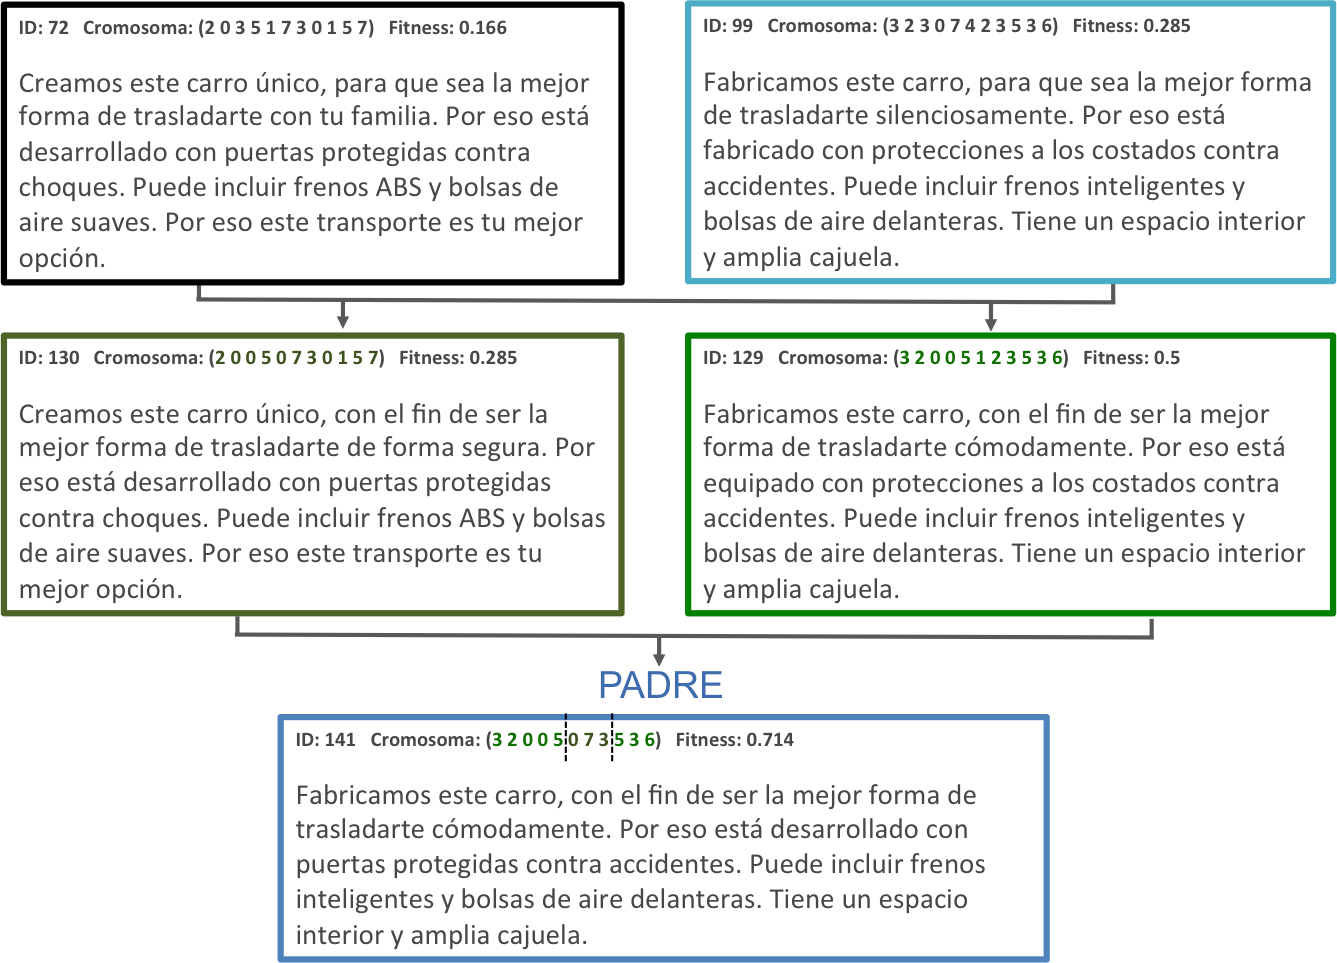
\includegraphics[width=7in]{p.png}} 
  \caption{Árbol Genealógico de un cromosoma (Parte del Padre)} 
\label{p}
\end{figure}

\begin{figure}[htp]
  \centerline{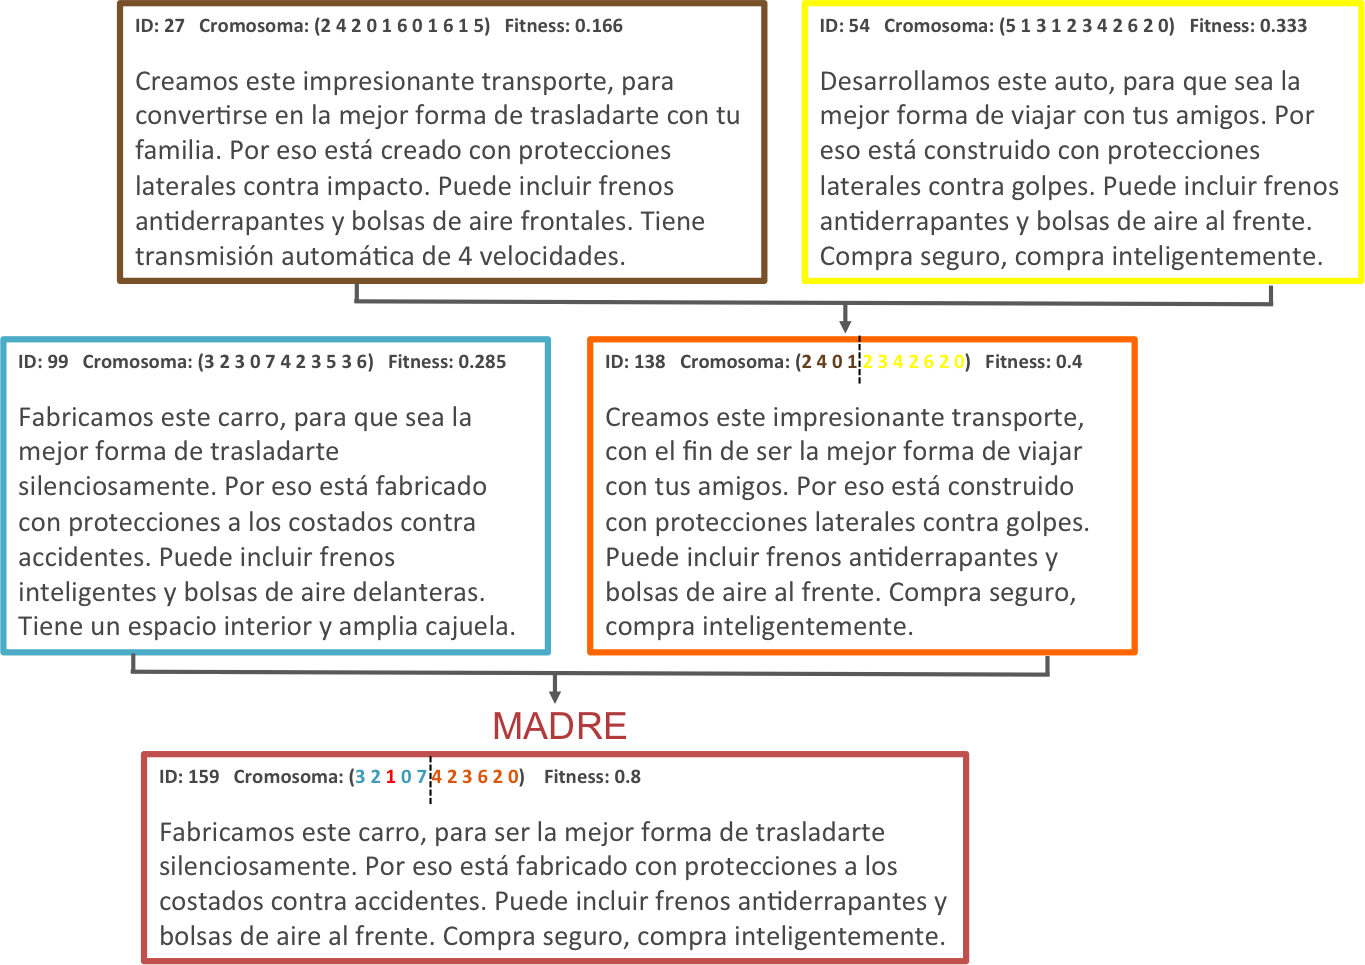
\includegraphics[width=7in]{m.png}} 
  \caption{Árbol Genealógico de un cromosoma (Parte del Madre)} 
\label{m}
\end{figure}

\clearpage
\newpage


\end{document}

